\documentclass{article} % A4 paper and 11pt font size
\setcounter{secnumdepth}{0}

\usepackage{multicol}
\usepackage{amssymb, amsmath, amsfonts}
\usepackage{moreverb}
\usepackage{multicol}
\usepackage{graphicx}
\usepackage{enumerate}
\usepackage{changepage}
\usepackage{lipsum}
\usepackage{caption}
\usepackage{nicefrac}
\usepackage{graphics}
\usepackage[margin=1in]{geometry}
\usepackage{tocloft}
\renewcommand{\cftsecleader}{\cftdotfill{\cftdotsep}}
\usepackage{array}
\usepackage{arydshln}
\usepackage{float}
\usepackage{subcaption}
\usepackage{csquotes}
\usepackage{placeins}
\usepackage{verbatim}
\usepackage{hyperref}
\usepackage{textcomp}
\usepackage[makeroom]{cancel}
\usepackage{bbold}
\usepackage{scrextend}
\usepackage{alltt}
\usepackage[utf8]{inputenc}
\usepackage{listings}
\usepackage{color}
\usepackage{physics}
\usepackage{mathtools}
\usepackage[normalem]{ulem}
\usepackage{amsthm}
\usepackage{tikz}
\usetikzlibrary{positioning}
\usetikzlibrary{arrows}
\usepackage{pgfplots}
\usepackage{bigints}
\allowdisplaybreaks
\pgfplotsset{compat=1.12}

\theoremstyle{plain}
\newtheorem*{theorem*}{Theorem}
\newtheorem{theorem}{Theorem}
\newtheorem*{lemma*}{Lemma}
\newtheorem{lemma}{Lemma}

\definecolor{verbgray}{gray}{0.9}
% \definecolor{dkgreen}{green}{0.9}

\lstdefinestyle{PythonCode}{%
  language=Python,
  backgroundcolor=\color{verbgray},
  keywordstyle=\color{blue},      % keyword style
  keywordstyle=[2]\color{blue},   % keyword style
  commentstyle=\color{magenta},   % comment style
  stringstyle=\color{olive},      % string literal styleframe=single,
  numberstyle=\color{black},      % string literal styleframe=single,
  framerule=0pt,
  numbers=left,
  stepnumber=1,
  firstnumber=1,
  showspaces=false,
  basicstyle=\ttfamily}

\lstset{style=PythonCode}

\makeatletter
\newcommand{\BIGG}{\bBigg@{3}}
\newcommand{\vast}{\bBigg@{4}}
\newcommand{\Vast}{\bBigg@{5}}
\makeatother

\newenvironment{definition}[1][Definition]{\begin{trivlist}
\item[\hskip \labelsep {\bfseries #1}]}{\end{trivlist}}

\newcommand{\dy}{\partial_y}
\newcommand{\dyy}{\partial_{yy}}
\newcommand{\dxx}{\partial_{xx}}
\newcommand{\dxy}{\partial_{xy}}
\newcommand{\dyyy}{\partial_{yyy}}
\newcommand{\dxxx}{\partial_{xxx}}
\newcommand{\dx}{\partial_x}
\newcommand{\E}{\varepsilon}
\def\Rl{\mathbb{R}}
\def\Cx{\mathbb{C}}

\newcommand{\Ei}{\text{Ei}}

\usepackage[T1]{fontenc} % Use 8-bit encoding that has 256 glyphs
\usepackage{fourier} % Use the Adobe Utopia font for the document - comment this line to return to the LaTeX default
\usepackage[english]{babel} % English language/hyphenation

\usepackage{sectsty} % Allows customizing section commands
\allsectionsfont{\centering \normalfont\scshape} % Make all sections centered, the default font and small caps

\usepackage{fancyhdr} % Custom headers and footers
\pagestyle{fancy} % Makes all pages in the document conform to the custom headers and footers
\fancyhead[L]{\bf Sam Fleischer}
\fancyhead[C]{\bf UC Davis \\ Numerical Solutions of Differential Equations (MAT228B)} % No page header - if you want one, create it in the same way as the footers below
\fancyhead[R]{\bf Winter 2017}

\fancyfoot[L]{\bf } % Empty left footer
\fancyfoot[C]{\bf \thepage} % Empty center footer
\fancyfoot[R]{\bf } % Page numbering for right footer
\renewcommand{\headrulewidth}{0pt} % Remove header underlines
\renewcommand{\footrulewidth}{0pt} % Remove footer underlines
\setlength{\headheight}{25pt} % Customize the height of the header

\newcommand{\VEC}[2]{\left\langle #1, #2 \right\rangle}
\newcommand{\ran}{\text{\rm ran }}
\newcommand{\Hilb}{\mathcal{H}}
\newcommand{\lap}{\Delta}

\newcommand{\Dx}{\Delta x}
\newcommand{\Dt}{\Delta t}

\newcommand{\littleo}[1]{\text{\scriptsize$\mathcal{O}$}\qty(#1)}

\DeclareMathOperator*{\esssup}{\text{ess~sup}}

\newcommand{\problem}[2]{
\vspace{.375cm}
\boxed{\begin{minipage}{\textwidth}
    \section{\bf #1}
    #2
\end{minipage}}
}

\numberwithin{equation}{section} % Number equations within sections (i.e. 1.1, 1.2, 2.1, 2.2 instead of 1, 2, 3, 4)
\numberwithin{figure}{section} % Number figures within sections (i.e. 1.1, 1.2, 2.1, 2.2 instead of 1, 2, 3, 4)
\numberwithin{table}{section} % Number tables within sections (i.e. 1.1, 1.2, 2.1, 2.2 instead of 1, 2, 3, 4)

\setlength\parindent{0pt} % Removes all indentation from paragraphs - comment this line for an assignment with lots of text

\newcommand{\horrule}[1]{\rule{\linewidth}{#1}} % Create horizontal rule command with 1 argument of height

\title{ 
\normalfont \normalsize 
\textsc{UC Davis, Numerical Solutions of Differential Equations (MAT 228B), Winter 2017} \\ [25pt] % Your university, school and/or department name(s)
\horrule{2pt} \\[01.4cm] % Thin top horizontal rule
\Huge Homework \#3 \\ % The assignment title
\horrule{2pt} \\[0.5cm] % Thick bottom horizontal rule
}

\author{\huge Sam Fleischer} % Your name

\date{March 3, 2017} % Today's date or a custom date

\begin{document}\thispagestyle{empty}

\maketitle % Print the title

\makeatletter
\@starttoc{toc}
\makeatother

\pagebreak

\problem{Problem 1}{Write programs to solve $$u_t + au_x = 0,$$ on $[0,1]$ with periodic boundary conditions using upwinding and Lax-Wendroff.  For smooth solutions we expect upwinding to be first-order accurate and Lax-Wendroff to be second-order accurate, but it is not clear what accuracy to expect for nonsmooth solutions.
\begin{enumerate}[\ \ (a)]
    \item Let $a = 1$ and solve the problem up to time $t = 1$.  Perform a refinement study for both upwinding and Lax-Wendroff with $\Dt = 0.9a\Dx$ with a smooth initial condition.  Compute the rate of convergence in the $1$-norm, $2$-norm, and max-norm.  Note that the exact solution at time $t = 1$ is the initial condition, and so computing the error is easy.
    \item Repeat the previous problem with the discontinuous initial condition
    \begin{align*}
        u(x,0) = \begin{cases} 1 & \text{if } \abs{x - \frac{1}{2}} < \frac{1}{4} \\ 0 & \text{otherwise} \end{cases}
    \end{align*}
\end{enumerate}}

Here are functions which make a sparse update matrix for upwinding and Law-Wendroff:
\lstinputlisting[language=Python, firstline=7, lastline=27]{operators.py}
where \verb|numpy| is imported as \verb|np| and \verb|scipy.sparse| is imported as \verb|sp|.  Here are methods which construct functions to apply the upwind or Lax-Wendroff matrices:
\lstinputlisting[language=Python, firstline=44, lastline=68]{operators.py}
Here are functions defining smooth or discontinuous initial conditions given a vector of $x$ values:
\lstinputlisting[language=Python, firstline=1, lastline=5]{code_for_homework.py}
Finally, here is sample code to solve a problem:
\lstinputlisting[language=Python, firstline=7, lastline=24]{code_for_homework.py}
Note that line 9 would change to \verb|step = make_LW_method(Nx,dx,dt,transport_coef)| if we wanted to use Lax-Wendroff instead of upwinding.


\begin{enumerate}[\ \ (a)]
    \item {\color{white}q}
        \begin{table}[ht!]
            \caption*{Upwinding, $a = 1$, $N_x = 0.9aN_t$, smooth initial condition: $u_0(x) = \frac{1}{2}\sin(2\pi x) + \frac{1}{2}$}
            \centering
            \begin{tabular}{||c|c|c||c|c||c|c||}\hline\hline
               $N_x$ & $\norm{u^{N_t} - u^0}_1$ & $\frac{\norm{u_\text{fine}^{N_t} - u_\text{fine}^0}_1}{\norm{u_\text{coarse}^{N_t} - u_\text{coarse}^0}_1}$ & $\norm{u^{N_t} - u^0}_2$ & $\frac{\norm{u_\text{fine}^{N_t} - u_\text{fine}^0}_2}{\norm{u_\text{coarse}^{N_t} - u_\text{coarse}^0}_2}$ & $\norm{u^{N_t} - u^0}_\infty$ & $\frac{\norm{u_\text{fine}^{N_t} - u_\text{fine}^0}_\infty}{\norm{u_\text{coarse}^{N_t} - u_\text{coarse}^0}_\infty}$ \\
            \hline
                 9 & 0.105829    & -        & 0.0390366   & -        & 0.165393    & -        \\
                18 & 0.0462153   & 0.436698 & 0.0120953   & 0.309844 & 0.0722268   & 0.436698 \\
                36 & 0.0205959   & 0.445651 & 0.00381168  & 0.315138 & 0.0323139   & 0.447395 \\
                72 & 0.00955095  & 0.463731 & 0.0012501   & 0.327967 & 0.0149975   & 0.46412  \\
               144 & 0.00457416  & 0.478922 & 0.000423374 & 0.338671 & 0.00718442  & 0.479041 \\
               288 & 0.00223496  & 0.488606 & 0.000146277 & 0.345503 & 0.00351058  & 0.488638 \\
               576 & 0.00110423  & 0.494071 & 5.11036e-05 & 0.349363 & 0.00173451  & 0.49408  \\
              1152 & 0.000548774 & 0.496975 & 1.79586e-05 & 0.351415 & 0.000862011 & 0.496977 \\
              2304 & 0.000273548 & 0.498472 & 6.32992e-06 & 0.352473 & 0.000429689 & 0.498473 \\
              4608 & 0.000136564 & 0.499232 & 2.23453e-06 & 0.35301  & 0.000214515 & 0.499232 \\
              9216 & 6.82295e-05 & 0.499615 & 7.89416e-07 & 0.353281 & 0.000107175 & 0.499615 \\
             18432 & 3.41016e-05 & 0.499807 & 2.78993e-07 & 0.353417 & 5.35667e-05 & 0.499807 \\
             36864 & 1.70475e-05 & 0.499904 & 9.862e-08   & 0.353485 & 2.67782e-05 & 0.499904 \\
            \hline\hline
            \end{tabular}
        \end{table}
        \vspace{-0.25cm}
        \begin{table}[ht!]
            \centering
            \begin{tabular}{||c|c|c||}\hline\hline
               $N_x$ &   time (in seconds) &   ratio of times \\
            \hline
                 9 &            0.00081  &         -        \\
                18 &            0.000635 &         0.783951 \\
                36 &            0.000844 &         1.32913  \\
                72 &            0.00121  &         1.43365  \\
               144 &            0.002144 &         1.7719   \\
               288 &            0.003905 &         1.82136  \\
               576 &            0.007908 &         2.0251   \\
              1152 &            0.016155 &         2.04287  \\
              2304 &            0.047833 &         2.96088  \\
              4608 &            0.105026 &         2.19568  \\
              9216 &            0.320367 &         3.05036  \\
             18432 &            1.20162  &         3.75075  \\
             36864 &            4.20294  &         3.49773  \\
            \hline\hline
            \end{tabular}
        \end{table}
        \FloatBarrier
        \begin{table}[ht!]
            \caption*{Lax-Wendroff, $a = 1$, $N_x = 0.9aN_t$, smooth initial condition: $u_0(x) = \frac{1}{2}\sin(2\pi x) + \frac{1}{2}$}
            \centering
            \begin{tabular}{||c|c|c||c|c||c|c||}\hline\hline
               $N_x$ & $\norm{u^{N_t} - u^0}_1$ & $\frac{\norm{u_\text{fine}^{N_t} - u_\text{fine}^0}_1}{\norm{u_\text{coarse}^{N_t} - u_\text{coarse}^0}_1}$ & $\norm{u^{N_t} - u^0}_2$ & $\frac{\norm{u_\text{fine}^{N_t} - u_\text{fine}^0}_2}{\norm{u_\text{coarse}^{N_t} - u_\text{coarse}^0}_2}$ & $\norm{u^{N_t} - u^0}_\infty$ & $\frac{\norm{u_\text{fine}^{N_t} - u_\text{fine}^0}_\infty}{\norm{u_\text{coarse}^{N_t} - u_\text{coarse}^0}_\infty}$ \\
            \hline
                 9 & 0.0502105   & -        & 0.0186936   & -        & 0.0784707   & -        \\
                18 & 0.0106443   & 0.211994 & 0.00278917  & 0.149204 & 0.0166353   & 0.211994 \\
                36 & 0.00232186  & 0.218131 & 0.000429486 & 0.153984 & 0.00363858  & 0.218727 \\
                72 & 0.000532585 & 0.229379 & 6.97013e-05 & 0.16229  & 0.000836081 & 0.229782 \\
               144 & 0.000126933 & 0.238335 & 1.17484e-05 & 0.168553 & 0.000199357 & 0.238442 \\
               288 & 3.09433e-05 & 0.243776 & 2.02521e-06 & 0.172382 & 4.86038e-05 & 0.243803 \\
               576 & 7.63624e-06 & 0.246782 & 3.53404e-07 & 0.174503 & 1.19949e-05 & 0.246789 \\
              1152 & 1.89656e-06 & 0.248363 & 6.20647e-08 & 0.17562  & 2.9791e-06  & 0.248365 \\
              2304 & 4.72574e-07 & 0.249175 & 1.09354e-08 & 0.176193 & 7.42318e-07 & 0.249175 \\
              4608 & 1.17948e-07 & 0.249585 & 1.92991e-09 & 0.176484 & 1.85272e-07 & 0.249586 \\
              9216 & 2.94624e-08 & 0.249792 & 3.40881e-10 & 0.17663  & 4.62795e-08 & 0.249792 \\
             18432 & 7.36254e-09 & 0.249896 & 6.02347e-11 & 0.176703 & 1.15651e-08 & 0.249896 \\
             36864 & 1.84025e-09 & 0.249948 & 1.06459e-11 & 0.17674  & 2.89066e-09 & 0.249948 \\
            \hline\hline
            \end{tabular}
        \end{table}
        \vspace{-0.25cm}
        \begin{table}[ht!]
            \centering
            \begin{tabular}{||c|c|c||}\hline\hline
               $N_x$ & time (in seconds) & ratio of times \\
            \hline
                 9 &            0.000962 &         -        \\
                18 &            0.000733 &         0.761954 \\
                36 &            0.0012   &         1.63711  \\
                72 &            0.001797 &         1.4975   \\
               144 &            0.002363 &         1.31497  \\
               288 &            0.003883 &         1.64325  \\
               576 &            0.009921 &         2.55498  \\
              1152 &            0.020166 &         2.03266  \\
              2304 &            0.050557 &         2.50704  \\
              4608 &            0.126219 &         2.49657  \\
              9216 &            0.401252 &         3.17901  \\
             18432 &            1.49188  &         3.71805  \\
             36864 &            5.44029  &         3.64661  \\
            \hline\hline
            \end{tabular}
        \end{table}
        \FloatBarrier
        These results show that for upwinding with continuous data, the $1$-norm and $\infty$-norm converge to $0$ on the scale of the mesh refinement, that is, the ratios of norms approach $\frac{1}{2}$.  The $2$-norm ratios converge to $\frac{1}{2\sqrt{2}}$.  Using Lax-Wendroff, we double the rate of convergence across the board.  The $1$-norm and $\infty$-norm converge with a ratio of $\frac{1}{4}$ and the $2$-norm converges with a ratio of $\frac{1}{4\sqrt{2}}$.  There is a slight trade-off, however, since the Lax-Wendroff matrix has a non-zero band on the super-diagonal and an element in the bottom left corner, so the computations are slightly more expensive.

    \item {\color{white}q}
        \begin{table}[ht!]
            \caption*{Upwinding, $a = 1$, $N_x = 0.9aN_t$, $u_0(x) = \mathcal{X}_{(\frac{1}{4},\frac{3}{4})}$}
            \centering
            \begin{tabular}{||c|c|c||c|c||c|c||}\hline\hline
               $N_x$ & $\norm{u^{N_t} - u^0}_1$ & $\frac{\norm{u_\text{fine}^{N_t} - u_\text{fine}^0}_1}{\norm{u_\text{coarse}^{N_t} - u_\text{coarse}^0}_1}$ & $\norm{u^{N_t} - u^0}_2$ & $\frac{\norm{u_\text{fine}^{N_t} - u_\text{fine}^0}_2}{\norm{u_\text{coarse}^{N_t} - u_\text{coarse}^0}_2}$ & $\norm{u^{N_t} - u^0}_\infty$ & $\frac{\norm{u_\text{fine}^{N_t} - u_\text{fine}^0}_\infty}{\norm{u_\text{coarse}^{N_t} - u_\text{coarse}^0}_\infty}$ \\
                \hline
                 9 & 0.216964   & -        & 0.0836486   & -        & 0.386057 & -       \\
                18 & 0.13819    & 0.636925 & 0.046883    & 0.560475 & 0.405849 & 1.05127 \\
                36 & 0.0913189  & 0.660821 & 0.0270755   & 0.577511 & 0.429004 & 1.05705 \\
                72 & 0.0621022  & 0.680059 & 0.0158358   & 0.584877 & 0.447831 & 1.04388 \\
               144 & 0.0429977  & 0.69237  & 0.00933364  & 0.589401 & 0.462319 & 1.03235 \\
               288 & 0.0300724  & 0.699397 & 0.00552469  & 0.591912 & 0.473056 & 1.02322 \\
               576 & 0.0211458  & 0.703161 & 0.00327744  & 0.593235 & 0.480838 & 1.01645 \\
              1152 & 0.0149101  & 0.70511  & 0.00194651  & 0.593913 & 0.486411 & 1.01159 \\
              2304 & 0.0105281  & 0.706103 & 0.00115673  & 0.594257 & 0.490377 & 1.00815 \\
              4608 & 0.00743916 & 0.706603 & 0.000687595 & 0.59443  & 0.493191 & 1.00574 \\
              9216 & 0.0052584  & 0.706855 & 0.000408786 & 0.594517 & 0.495183 & 1.00404 \\
             18432 & 0.00371759 & 0.706981 & 0.000243048 & 0.59456  & 0.496593 & 1.00285 \\
             36864 & 0.0026285  & 0.707044 & 0.000144512 & 0.594582 & 0.497591 & 1.00201 \\
             \hline\hline
            \end{tabular}
        \end{table}
        \vspace{-0.25cm}
        \begin{table}[ht!]
            \centering
            \begin{tabular}{||c|c|c||}\hline\hline
               $N_x$ & time (in seconds) & ratio of times \\
            \hline
                 9 &            0.000796 &         -        \\
                18 &            0.00076  &         0.954774 \\
                36 &            0.000954 &         1.25526  \\
                72 &            0.001379 &         1.44549  \\
               144 &            0.002448 &         1.7752   \\
               288 &            0.00472  &         1.9281   \\
               576 &            0.008401 &         1.77987  \\
              1152 &            0.019004 &         2.26211  \\
              2304 &            0.050015 &         2.63181  \\
              4608 &            0.121901 &         2.43729  \\
              9216 &            0.389288 &         3.19348  \\
             18432 &            1.71821  &         4.41373  \\
             36864 &            6.93595  &         4.03672  \\
             \hline\hline
            \end{tabular}
        \end{table}
        \FloatBarrier
        \begin{table}[ht!]
            \caption*{Lax-Wendroff, $a = 1$, $N_x = 0.9aN_t$, $u_0(x) = \mathcal{X}_{(\frac{1}{4},\frac{3}{4})}$}
            \centering
            \begin{tabular}{||c|c|c||c|c||c|c||}\hline\hline
               $N_x$ & $\norm{u^{N_t} - u^0}_1$ & $\frac{\norm{u_\text{fine}^{N_t} - u_\text{fine}^0}_1}{\norm{u_\text{coarse}^{N_t} - u_\text{coarse}^0}_1}$ & $\norm{u^{N_t} - u^0}_2$ & $\frac{\norm{u_\text{fine}^{N_t} - u_\text{fine}^0}_2}{\norm{u_\text{coarse}^{N_t} - u_\text{coarse}^0}_2}$ & $\norm{u^{N_t} - u^0}_\infty$ & $\frac{\norm{u_\text{fine}^{N_t} - u_\text{fine}^0}_\infty}{\norm{u_\text{coarse}^{N_t} - u_\text{coarse}^0}_\infty}$ \\
                \hline
                 9 & 0.158161   & -        & 0.070497    & -        & 0.391898 & -       \\
                18 & 0.123856   & 0.783104 & 0.041995    & 0.5957   & 0.435822 & 1.11208 \\
                36 & 0.0776195  & 0.62669  & 0.0238306   & 0.567462 & 0.475573 & 1.09121 \\
                72 & 0.049597   & 0.638977 & 0.0136343   & 0.572137 & 0.513524 & 1.0798  \\
               144 & 0.0321487  & 0.648197 & 0.00782582  & 0.573979 & 0.545926 & 1.0631  \\
               288 & 0.0212826  & 0.662006 & 0.00449387  & 0.574236 & 0.572148 & 1.04803 \\
               576 & 0.014095   & 0.662279 & 0.00257826  & 0.573728 & 0.592811 & 1.03611 \\
              1152 & 0.00929647 & 0.659557 & 0.00147713  & 0.572916 & 0.608913 & 1.02716 \\
              2304 & 0.00615957 & 0.662571 & 0.000844953 & 0.572024 & 0.621425 & 1.02055 \\
              4608 & 0.00406969 & 0.660709 & 0.000482597 & 0.571152 & 0.631154 & 1.01566 \\
              9216 & 0.00269564 & 0.66237  & 0.000275243 & 0.570338 & 0.638737 & 1.01201 \\
             18432 & 0.00178031 & 0.66044  & 0.000156777 & 0.569594 & 0.644664 & 1.00928 \\
             36864 & 0.00117545 & 0.660252 & 8.91934e-05 & 0.56892  & 0.649308 & 1.0072  \\
            \hline\hline
            \end{tabular}
        \end{table}
        \vspace{-0.25cm}
        \begin{table}[ht!]
            \centering
            \begin{tabular}{||c|c|c||}\hline\hline
               $N_x$ &   time (in seconds) &   ratio of times \\
            \hline
                 9 &            0.000949 &         -        \\
                18 &            0.000746 &         0.786091 \\
                36 &            0.000904 &         1.2118   \\
                72 &            0.001327 &         1.46792  \\
               144 &            0.002165 &         1.6315   \\
               288 &            0.004459 &         2.05958  \\
               576 &            0.007954 &         1.78381  \\
              1152 &            0.017039 &         2.14219  \\
              2304 &            0.048265 &         2.83262  \\
              4608 &            0.153822 &         3.18703  \\
              9216 &            0.664133 &         4.31754  \\
             18432 &            3.42794  &         5.16153  \\
             36864 &           15.8522   &         4.62441  \\
            \hline\hline
            \end{tabular}
        \end{table}
        \FloatBarrier
        These results show that for both upwinding and Lax-Wendroff, while the $1$-norm and $2$-norm ratios approach a number less than $1$ (suggesting convergence), the $\infty$-norm does not converge.  This is because there is a phase-shift for the high frequencies captured at the discontinuities.
\end{enumerate}

Below are images of the solutions.  The horizontal axis is time, with $t = 0$ on the left and $t = 1$ on the right.  The vertical axis is space, with $x_j = x_0$ on top and $x_j = x_{N_x}$ on bottom.  The first four images depict smooth initial data and the next four depict discontinuous initial data.  Notice the diffusion in the upwinding technique.  Even for smooth data, we see a loss of amplitude at $t = 1$.  Lax-Wendroff is very suited for continuous data - the red curve completely covers up the black curve.  When we use Lax-Wendroff for discontinuous data, we see a dark blue band and a white band moving slower (initially) than the rest of the data.  This is because high frequencies have a significant lag in the Lax-Wendroff method.  We don't see as much lag in the upwinding scheme for discontinuous data, but we do see significant diffusion because $g_\text{up-wind}(\xi)$ is relatively small.

\begin{figure}[ht!]
    \centering
    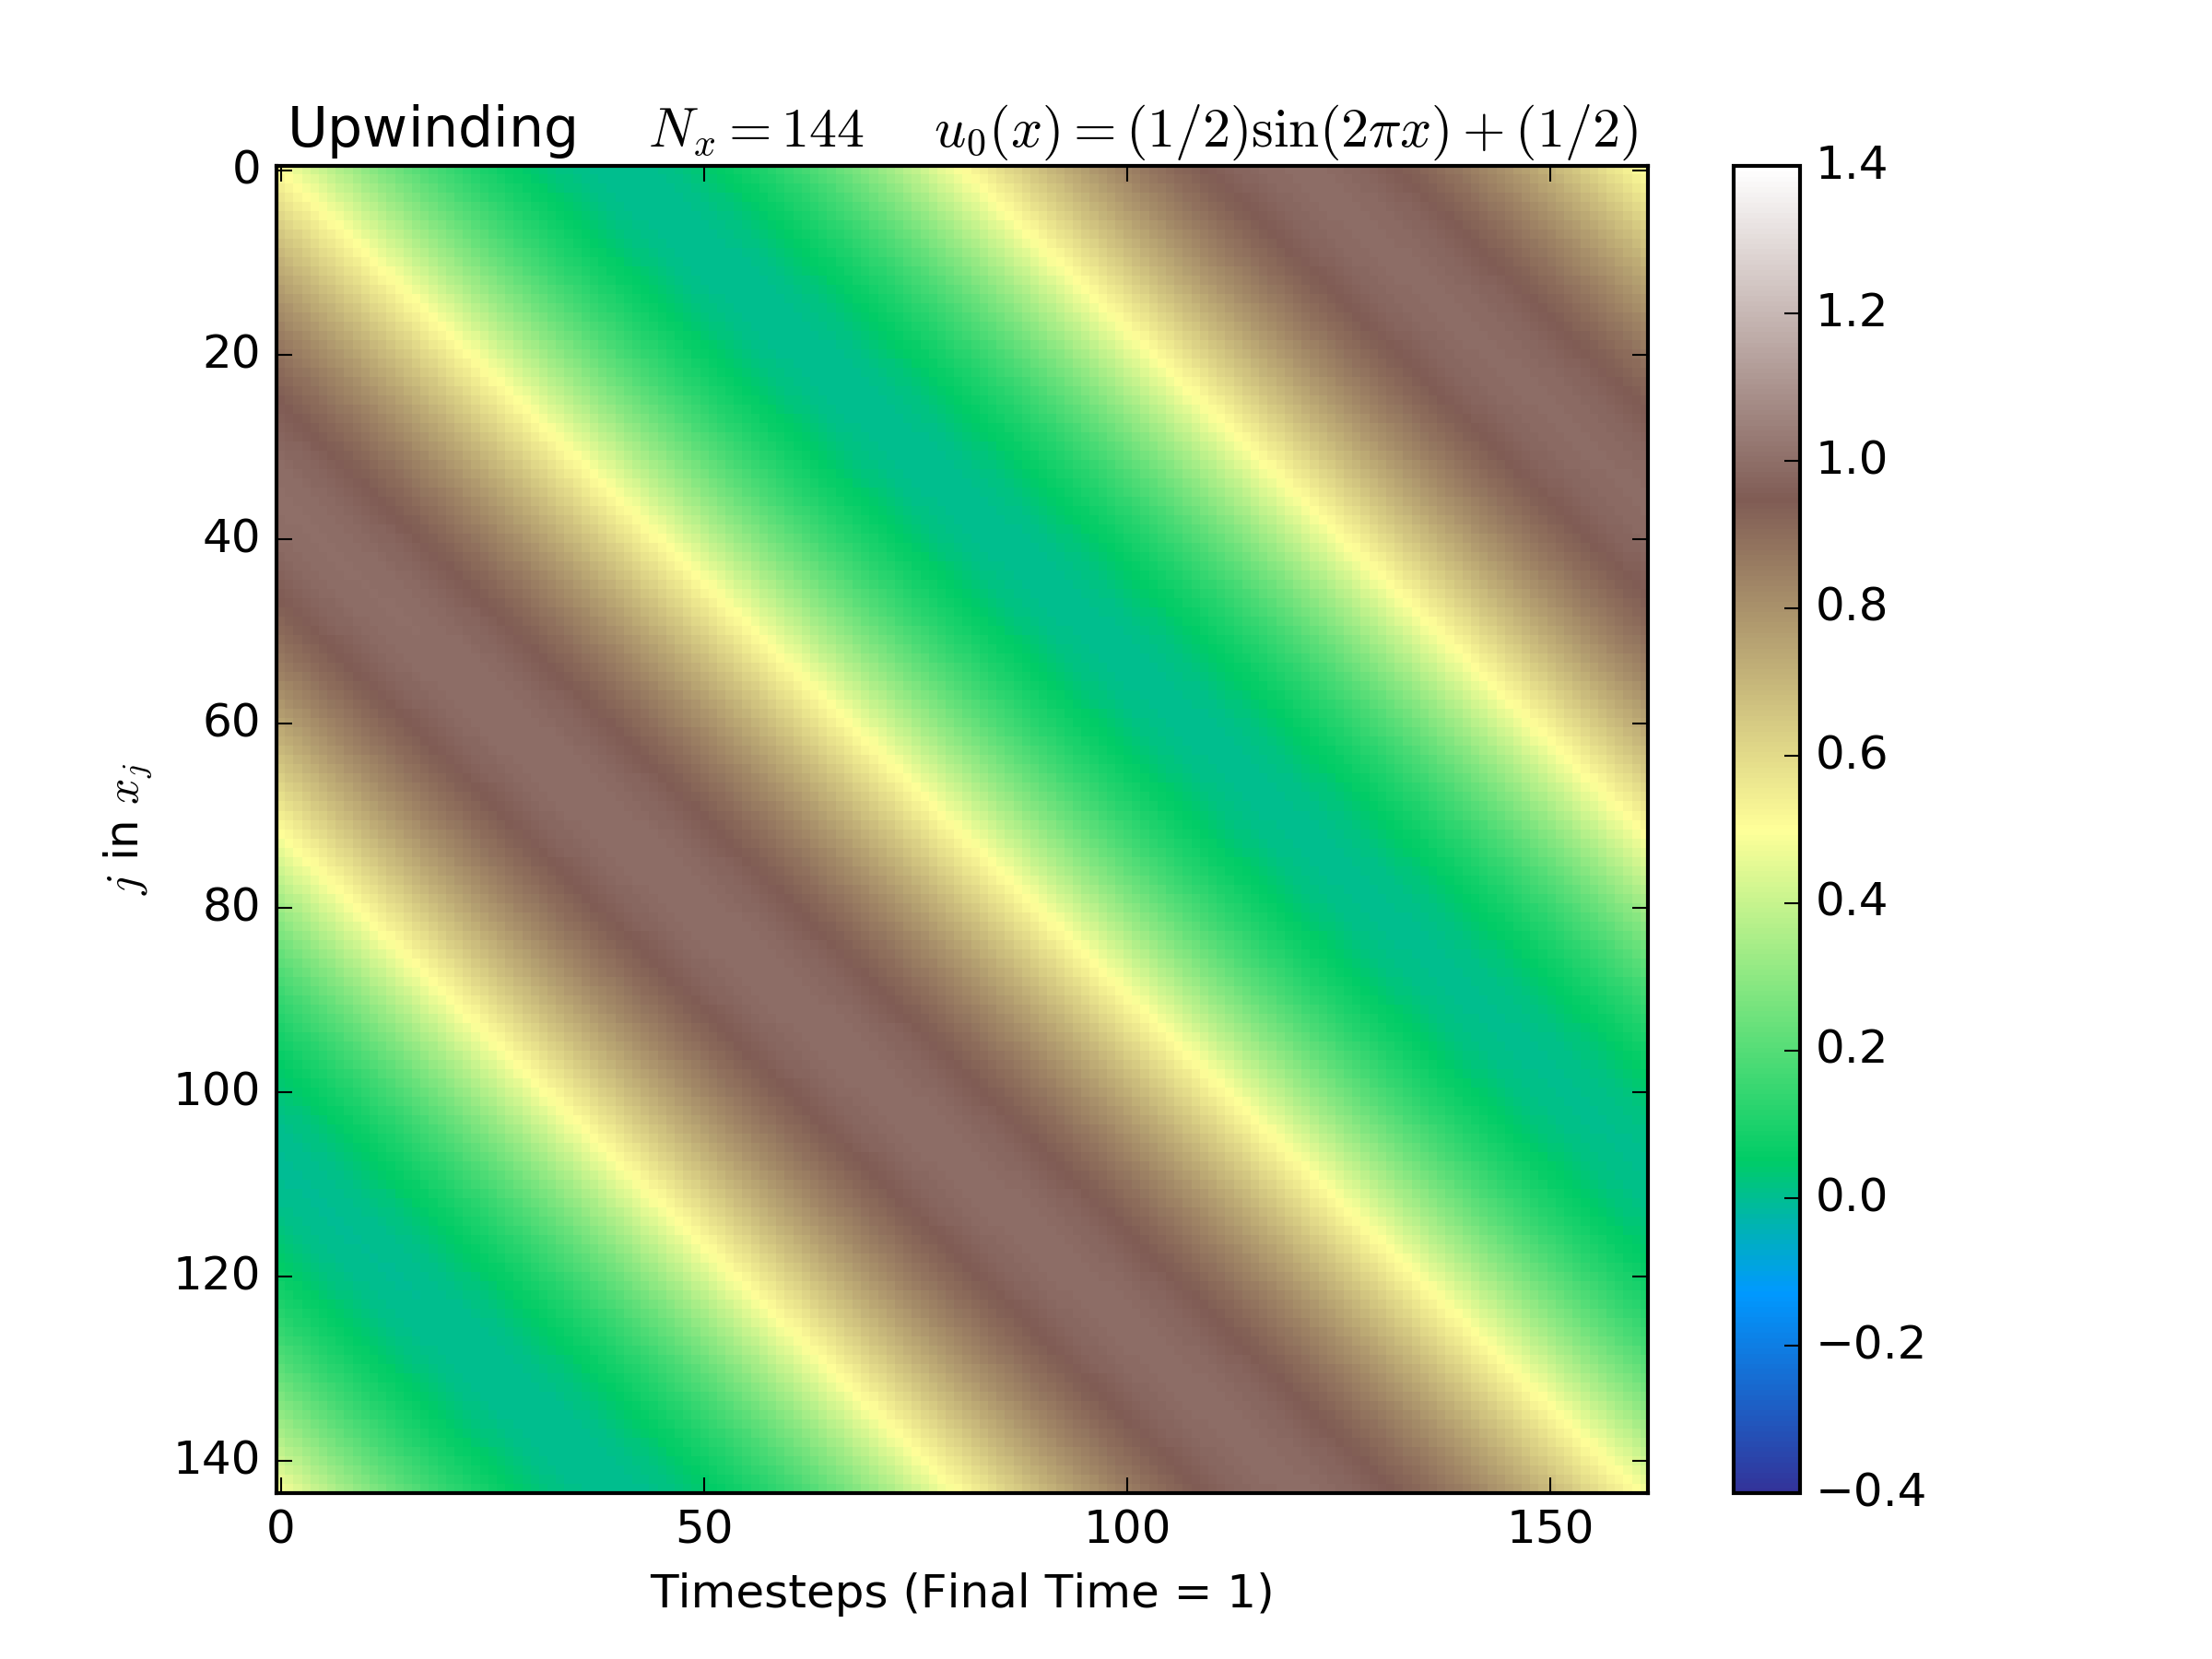
\includegraphics[width=0.45\textwidth]{figures/upwind_smooth.png}
    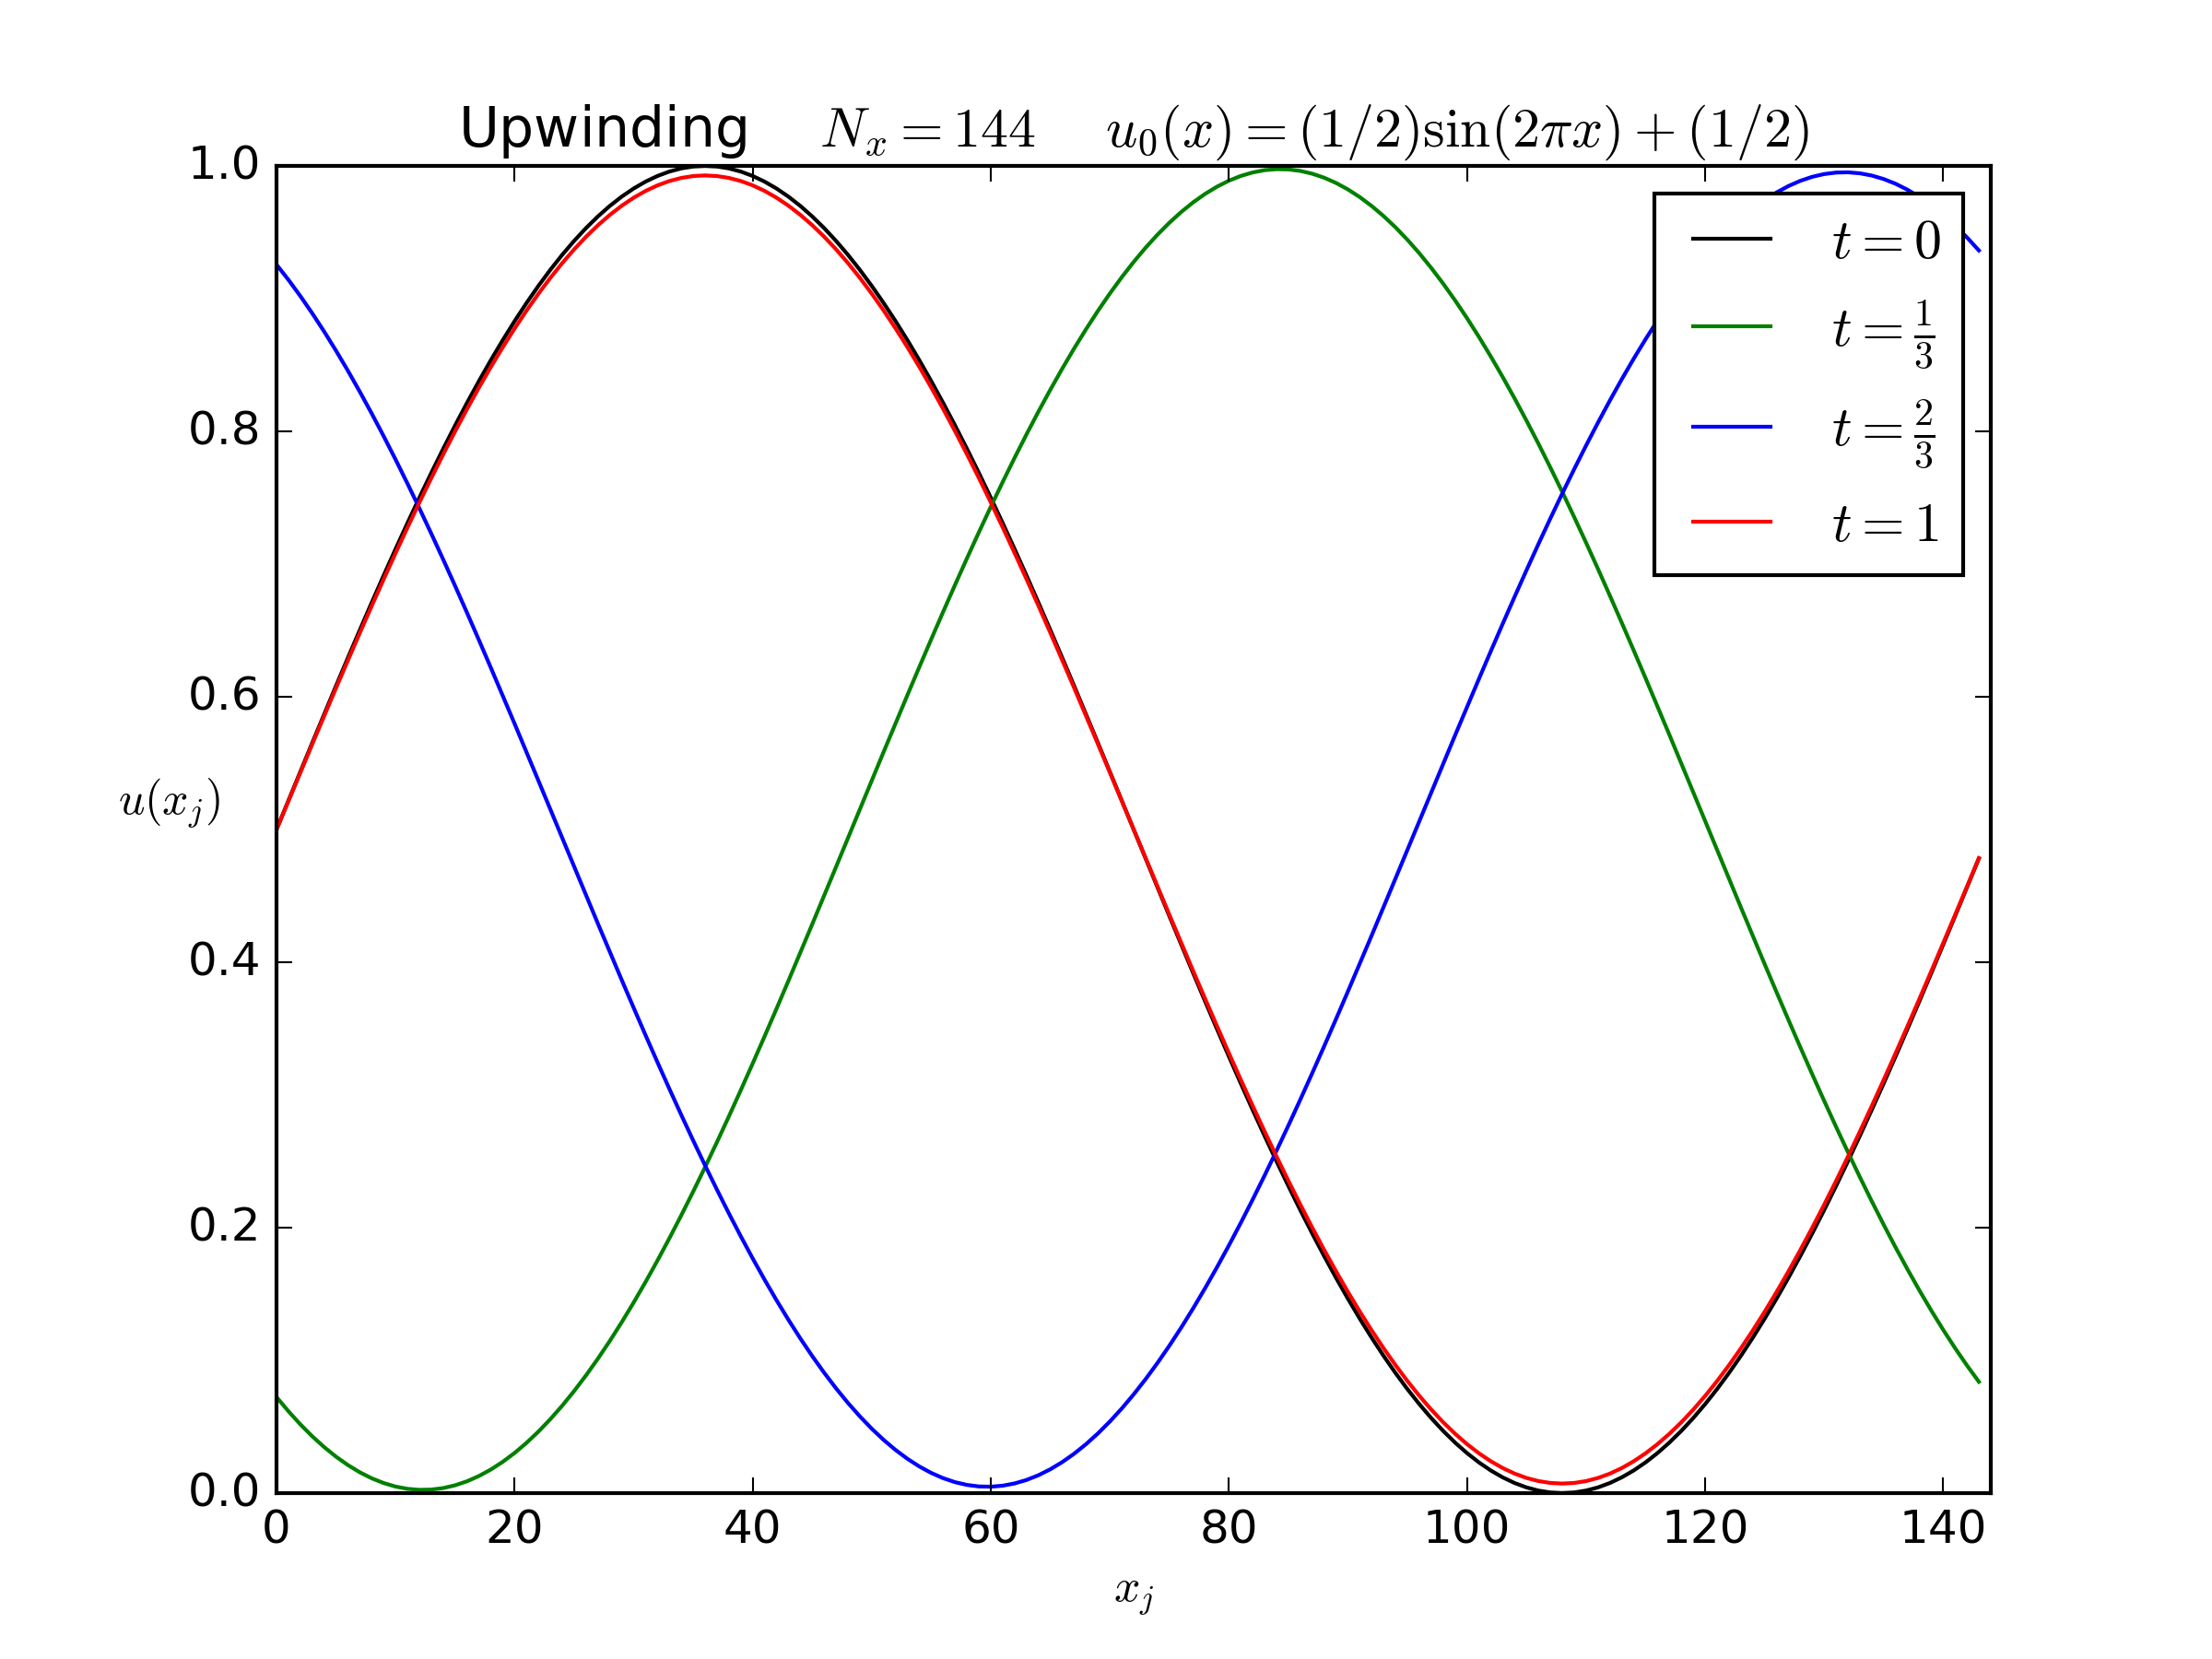
\includegraphics[width=0.45\textwidth]{figures/upwind_smooth_snapshots.png}
    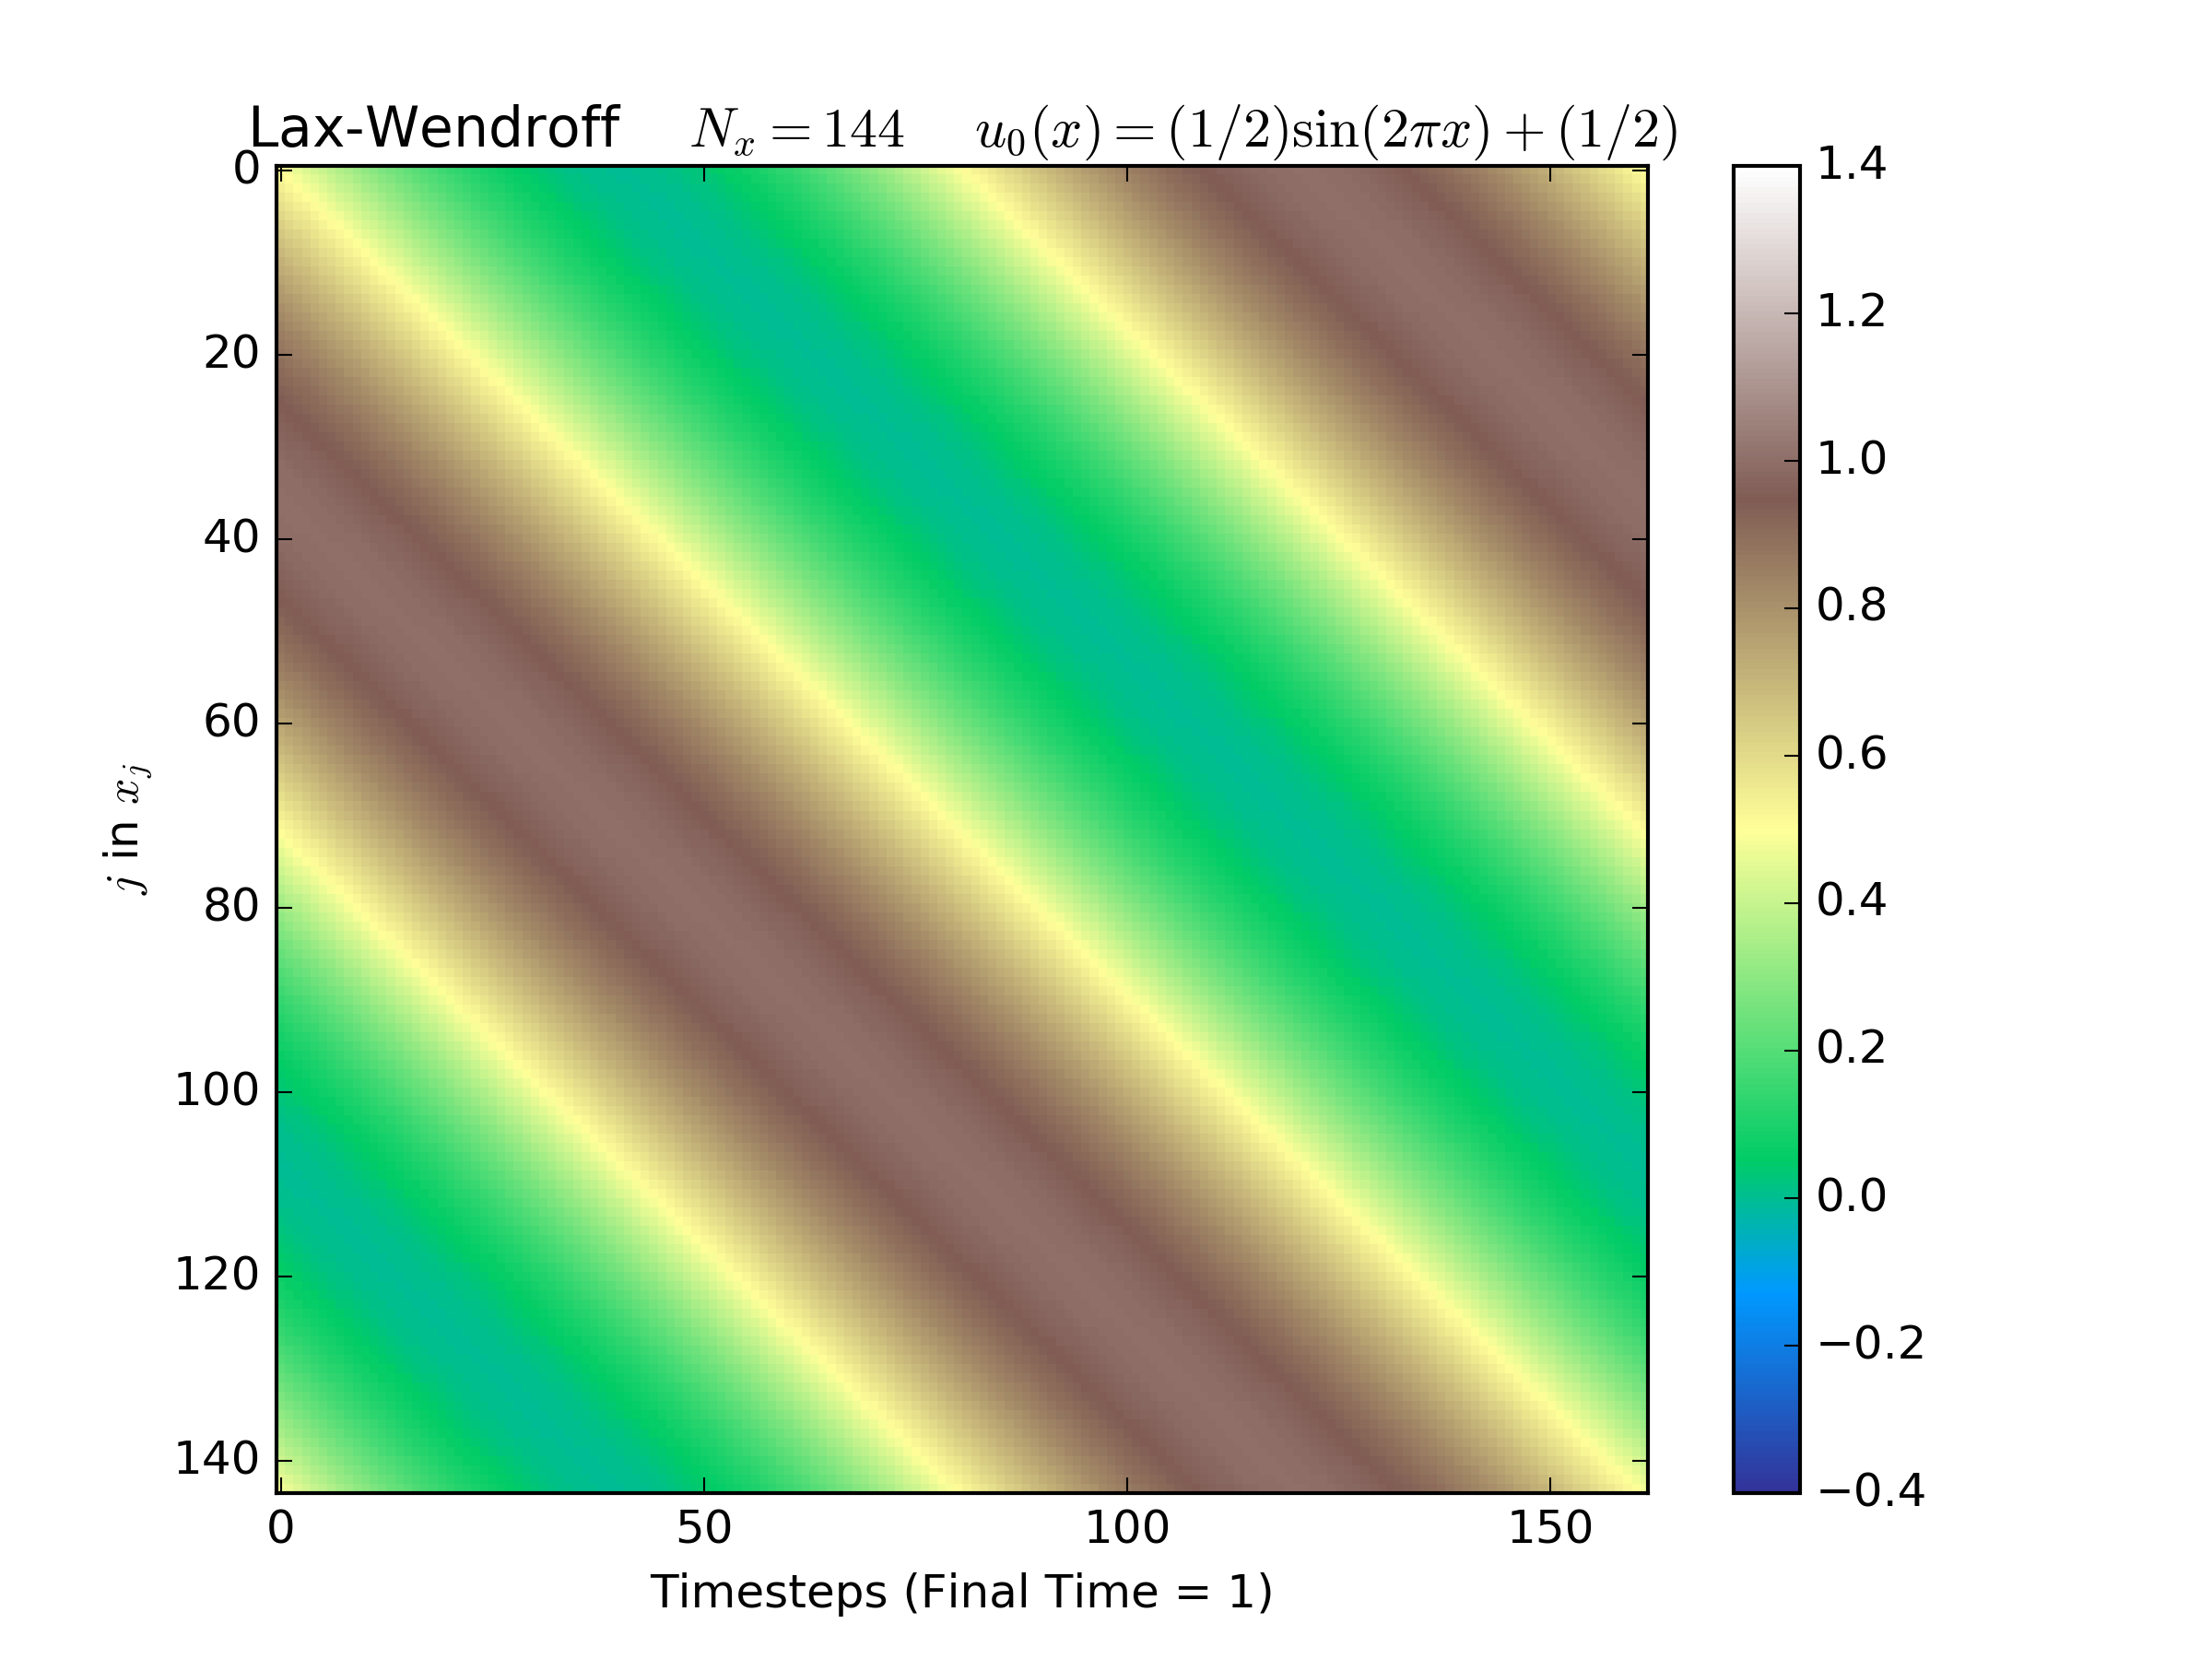
\includegraphics[width=0.45\textwidth]{figures/LW_smooth.png}
    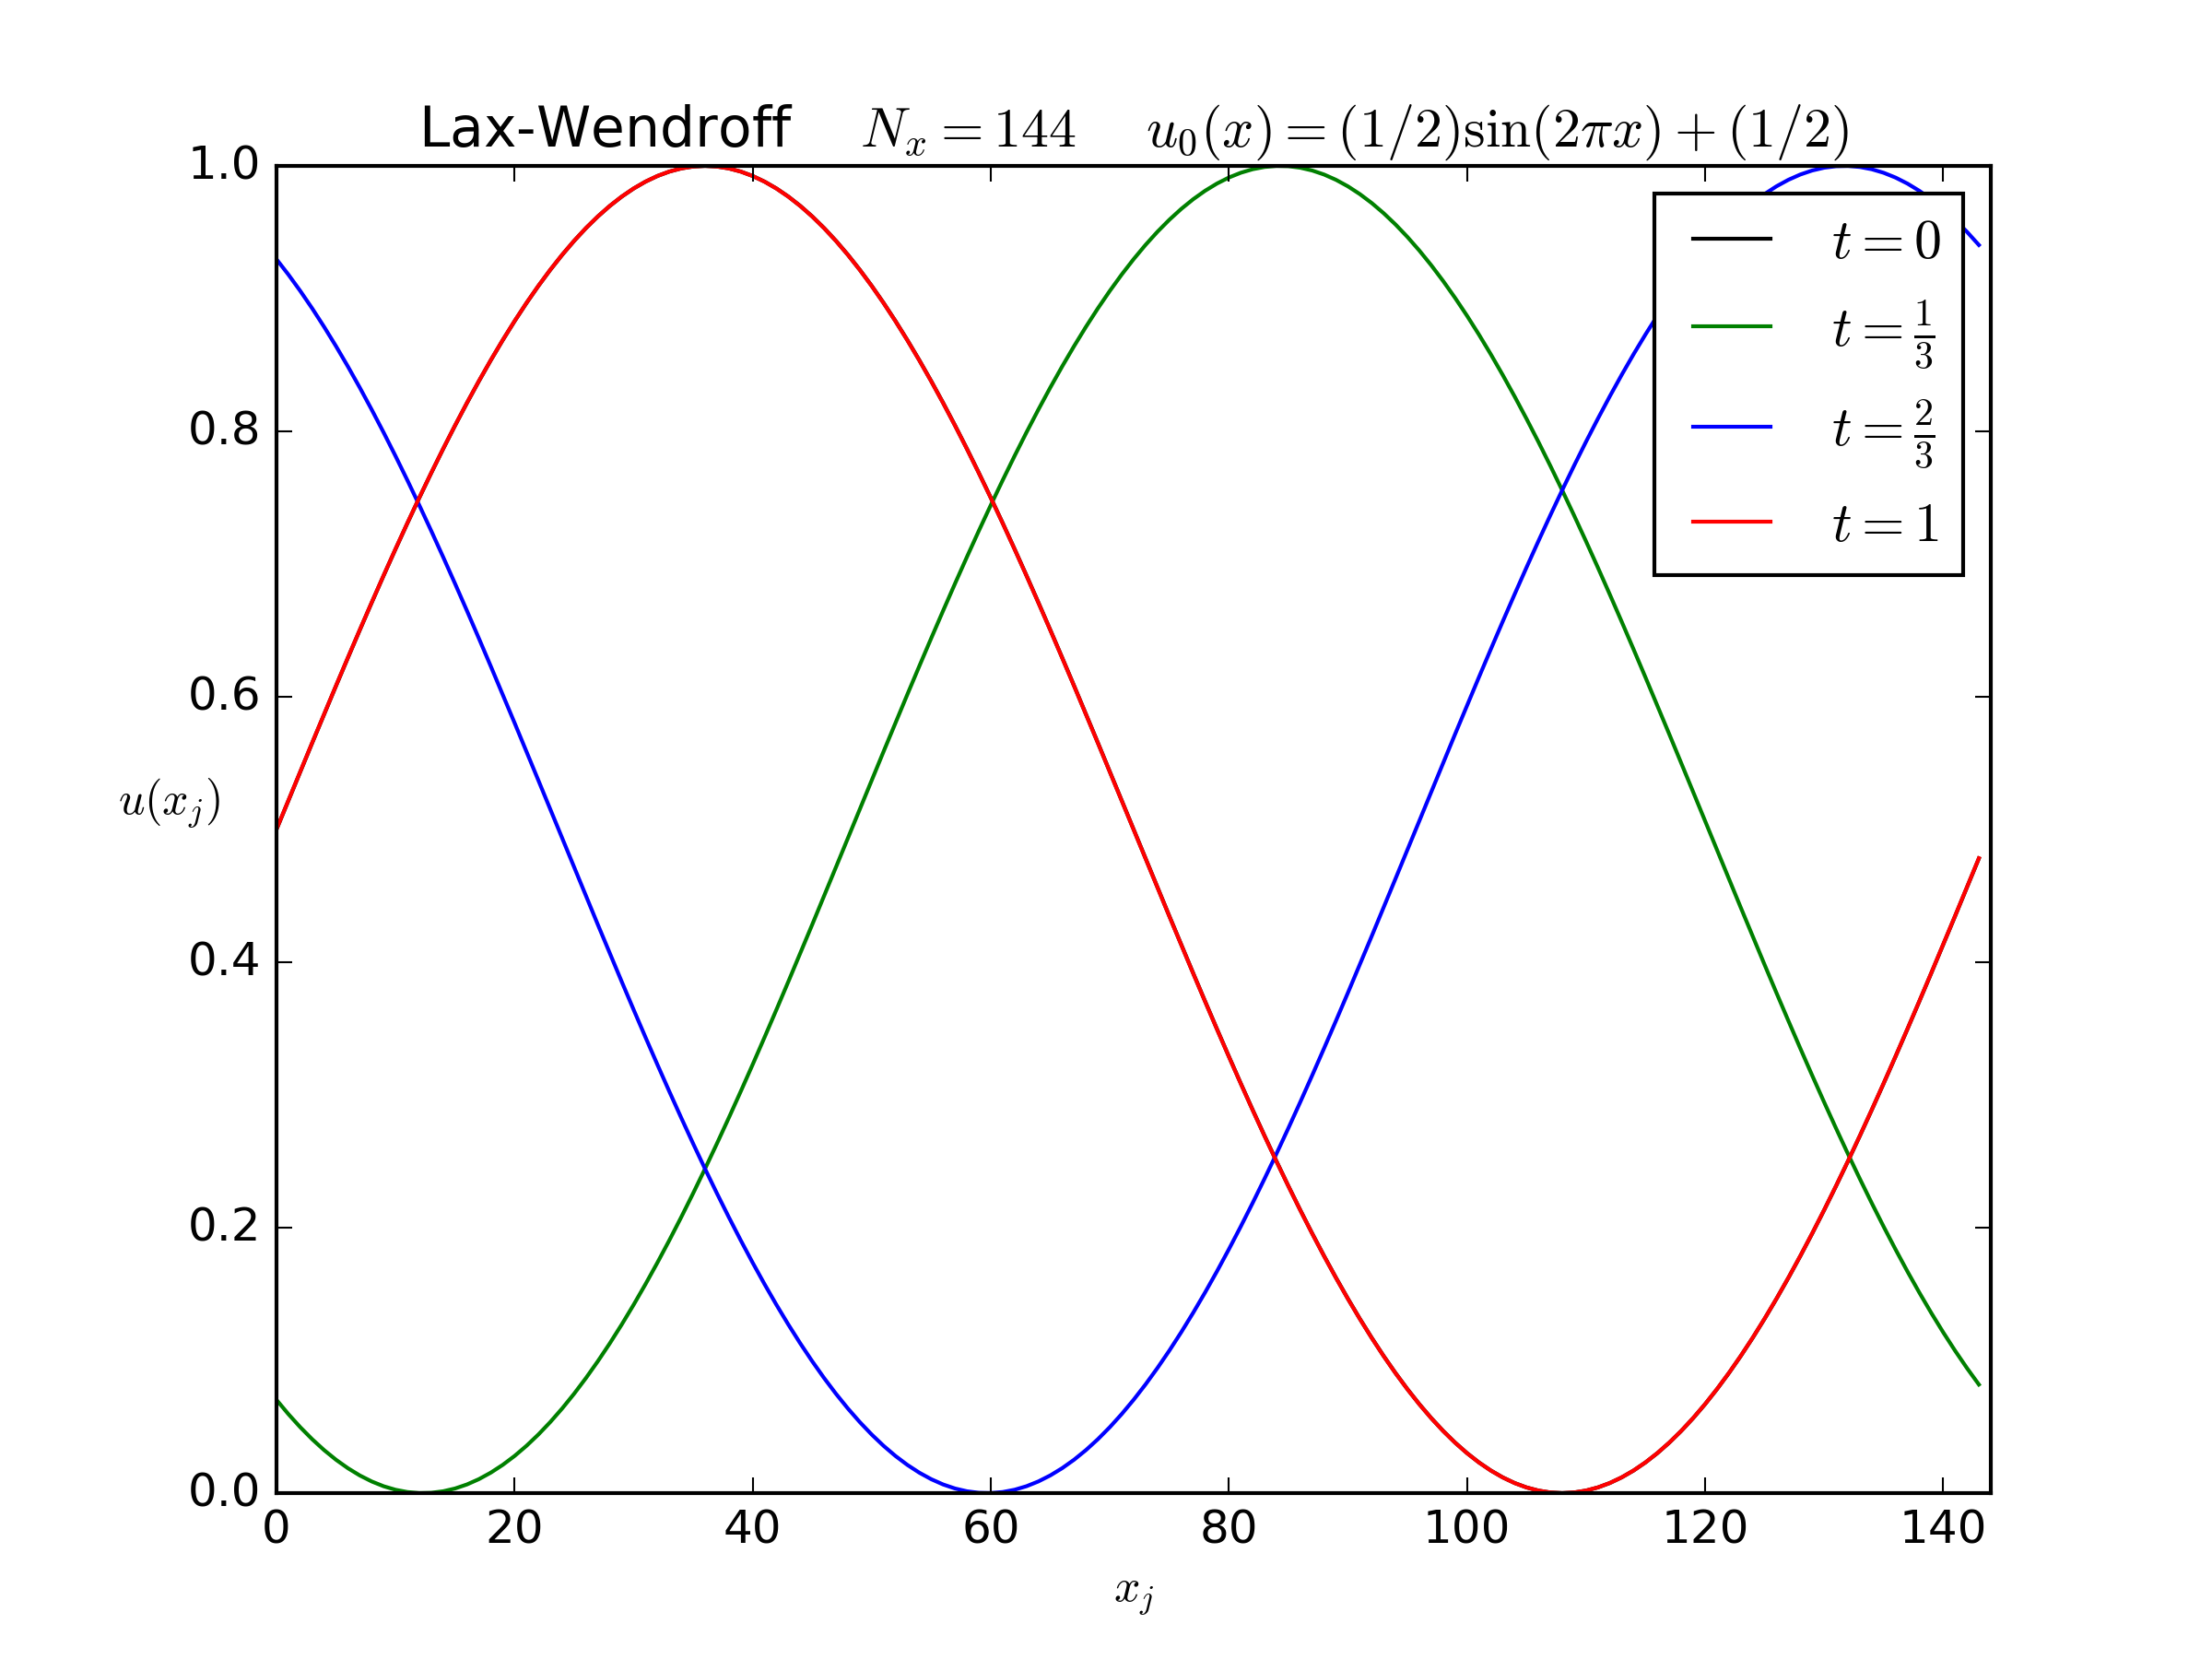
\includegraphics[width=0.45\textwidth]{figures/LW_smooth_snapshots.png}
    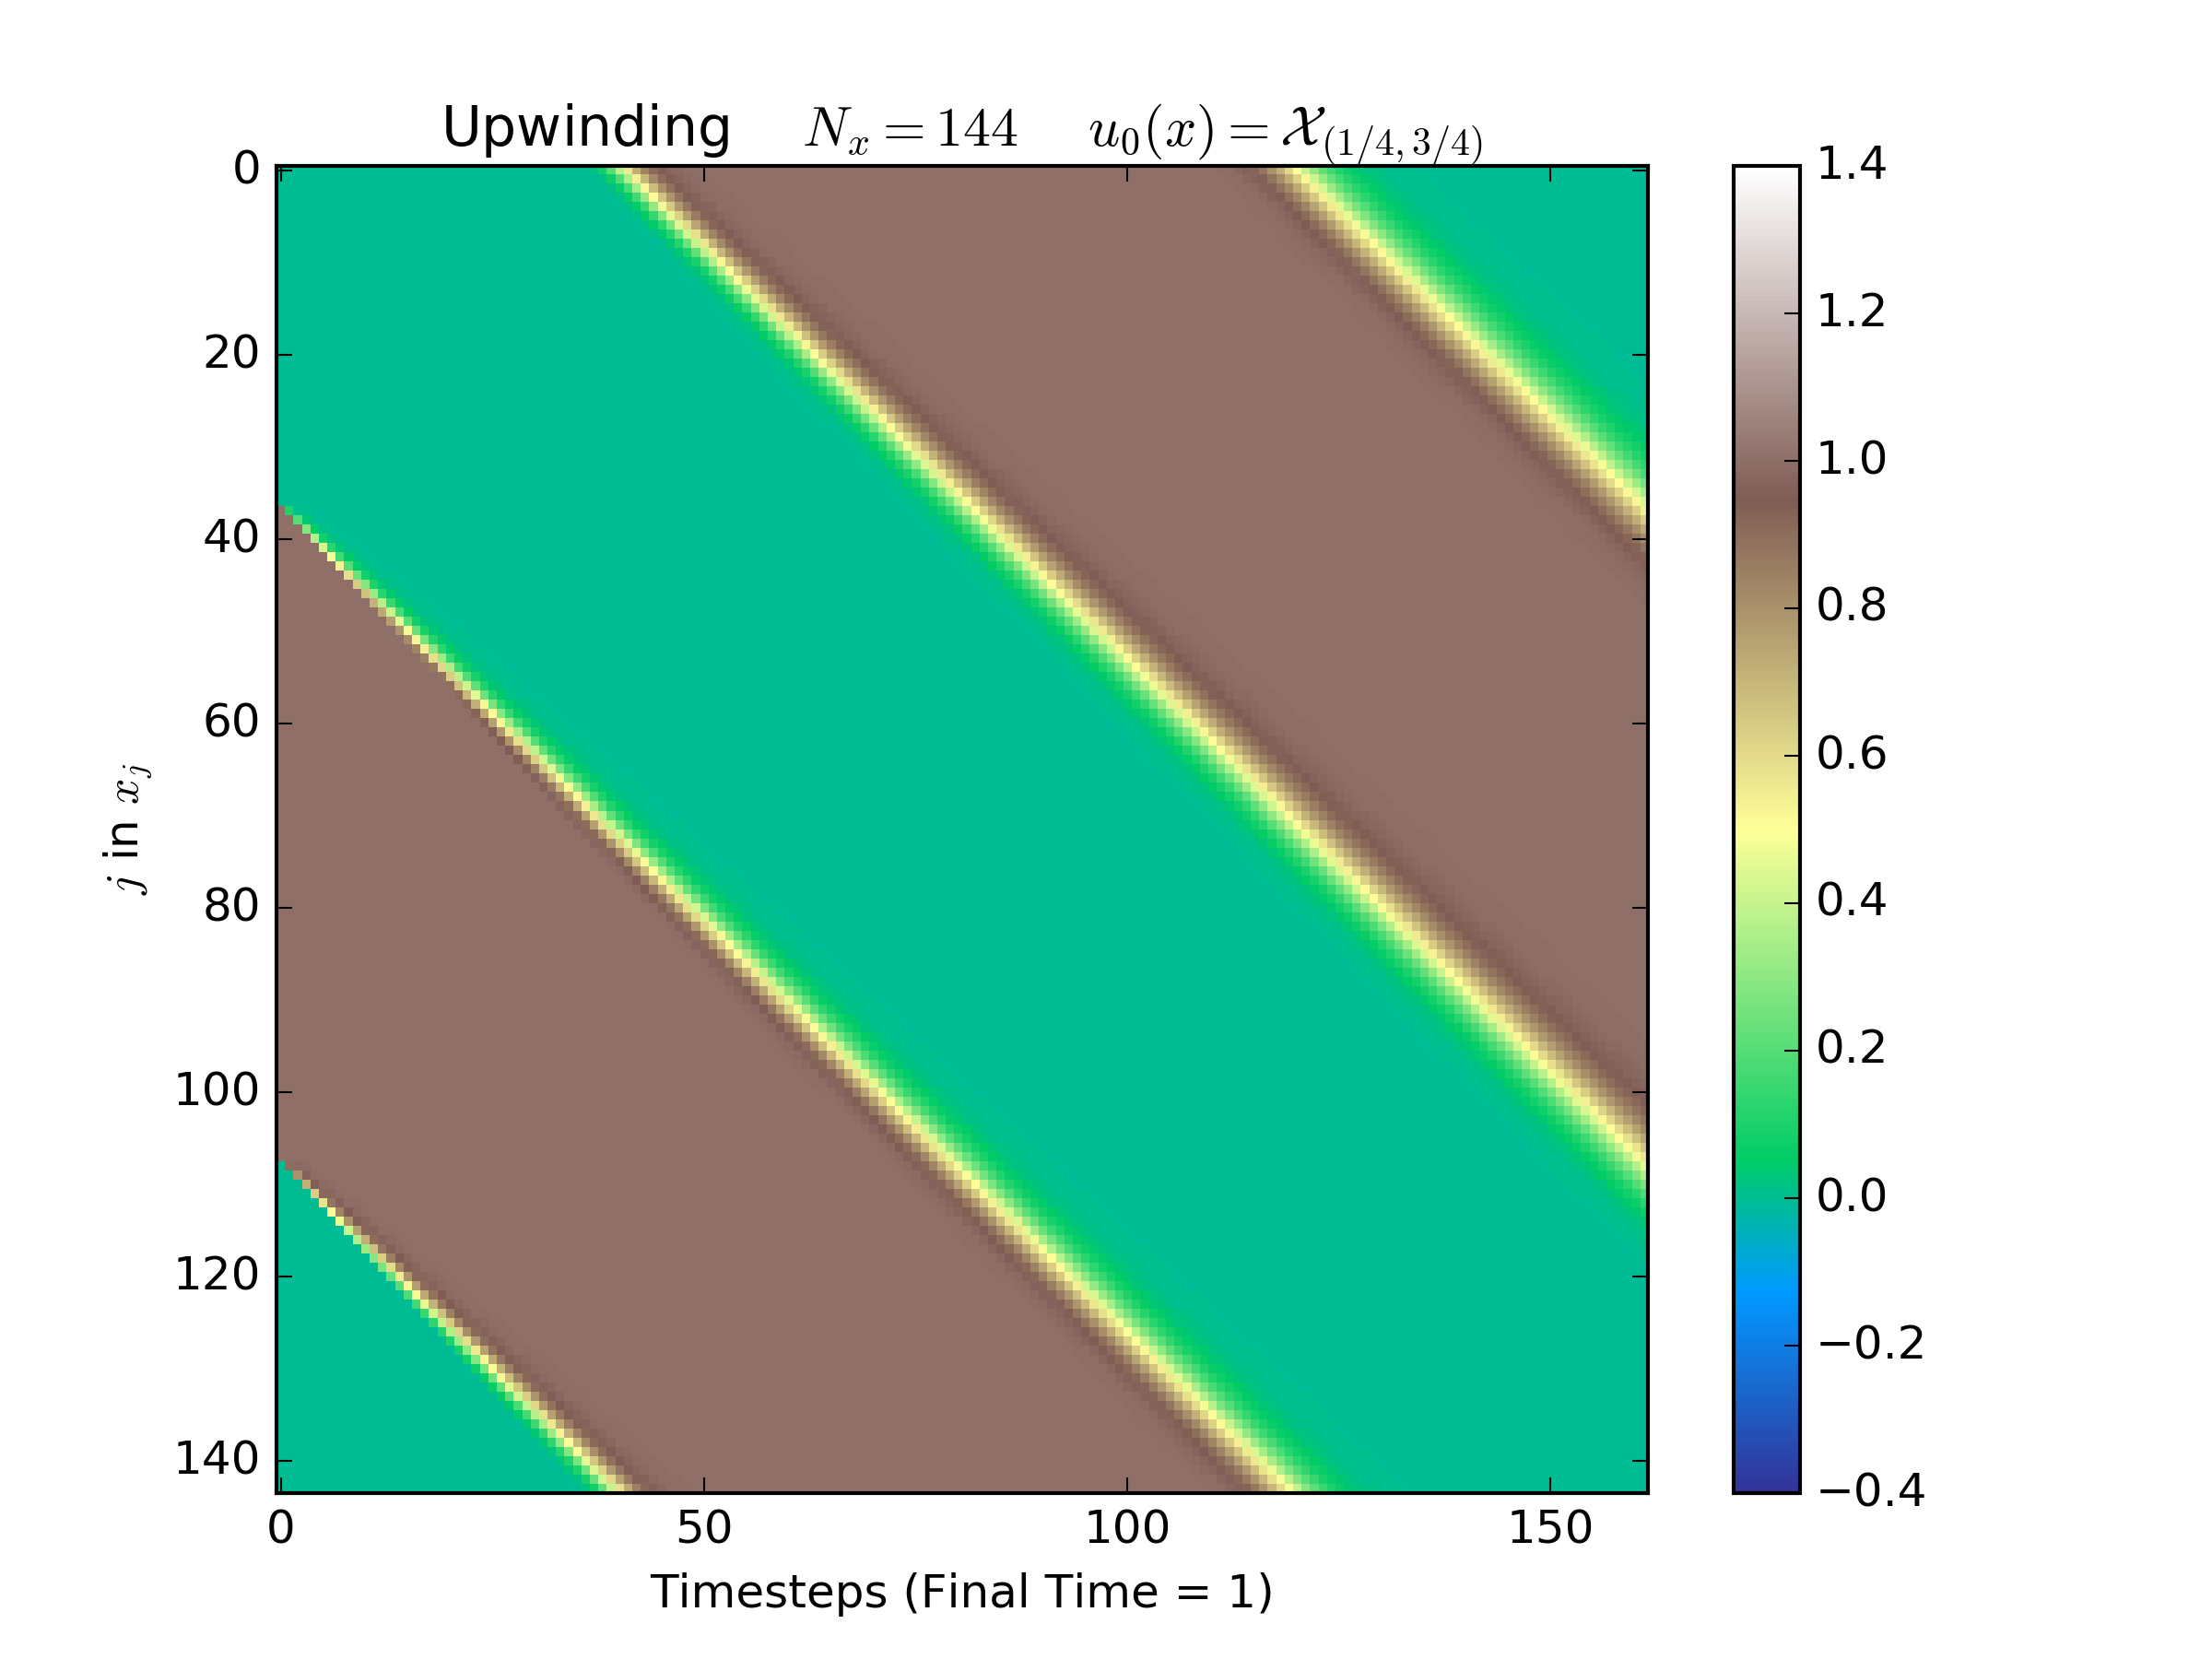
\includegraphics[width=0.45\textwidth]{figures/upwind_discon.png}
    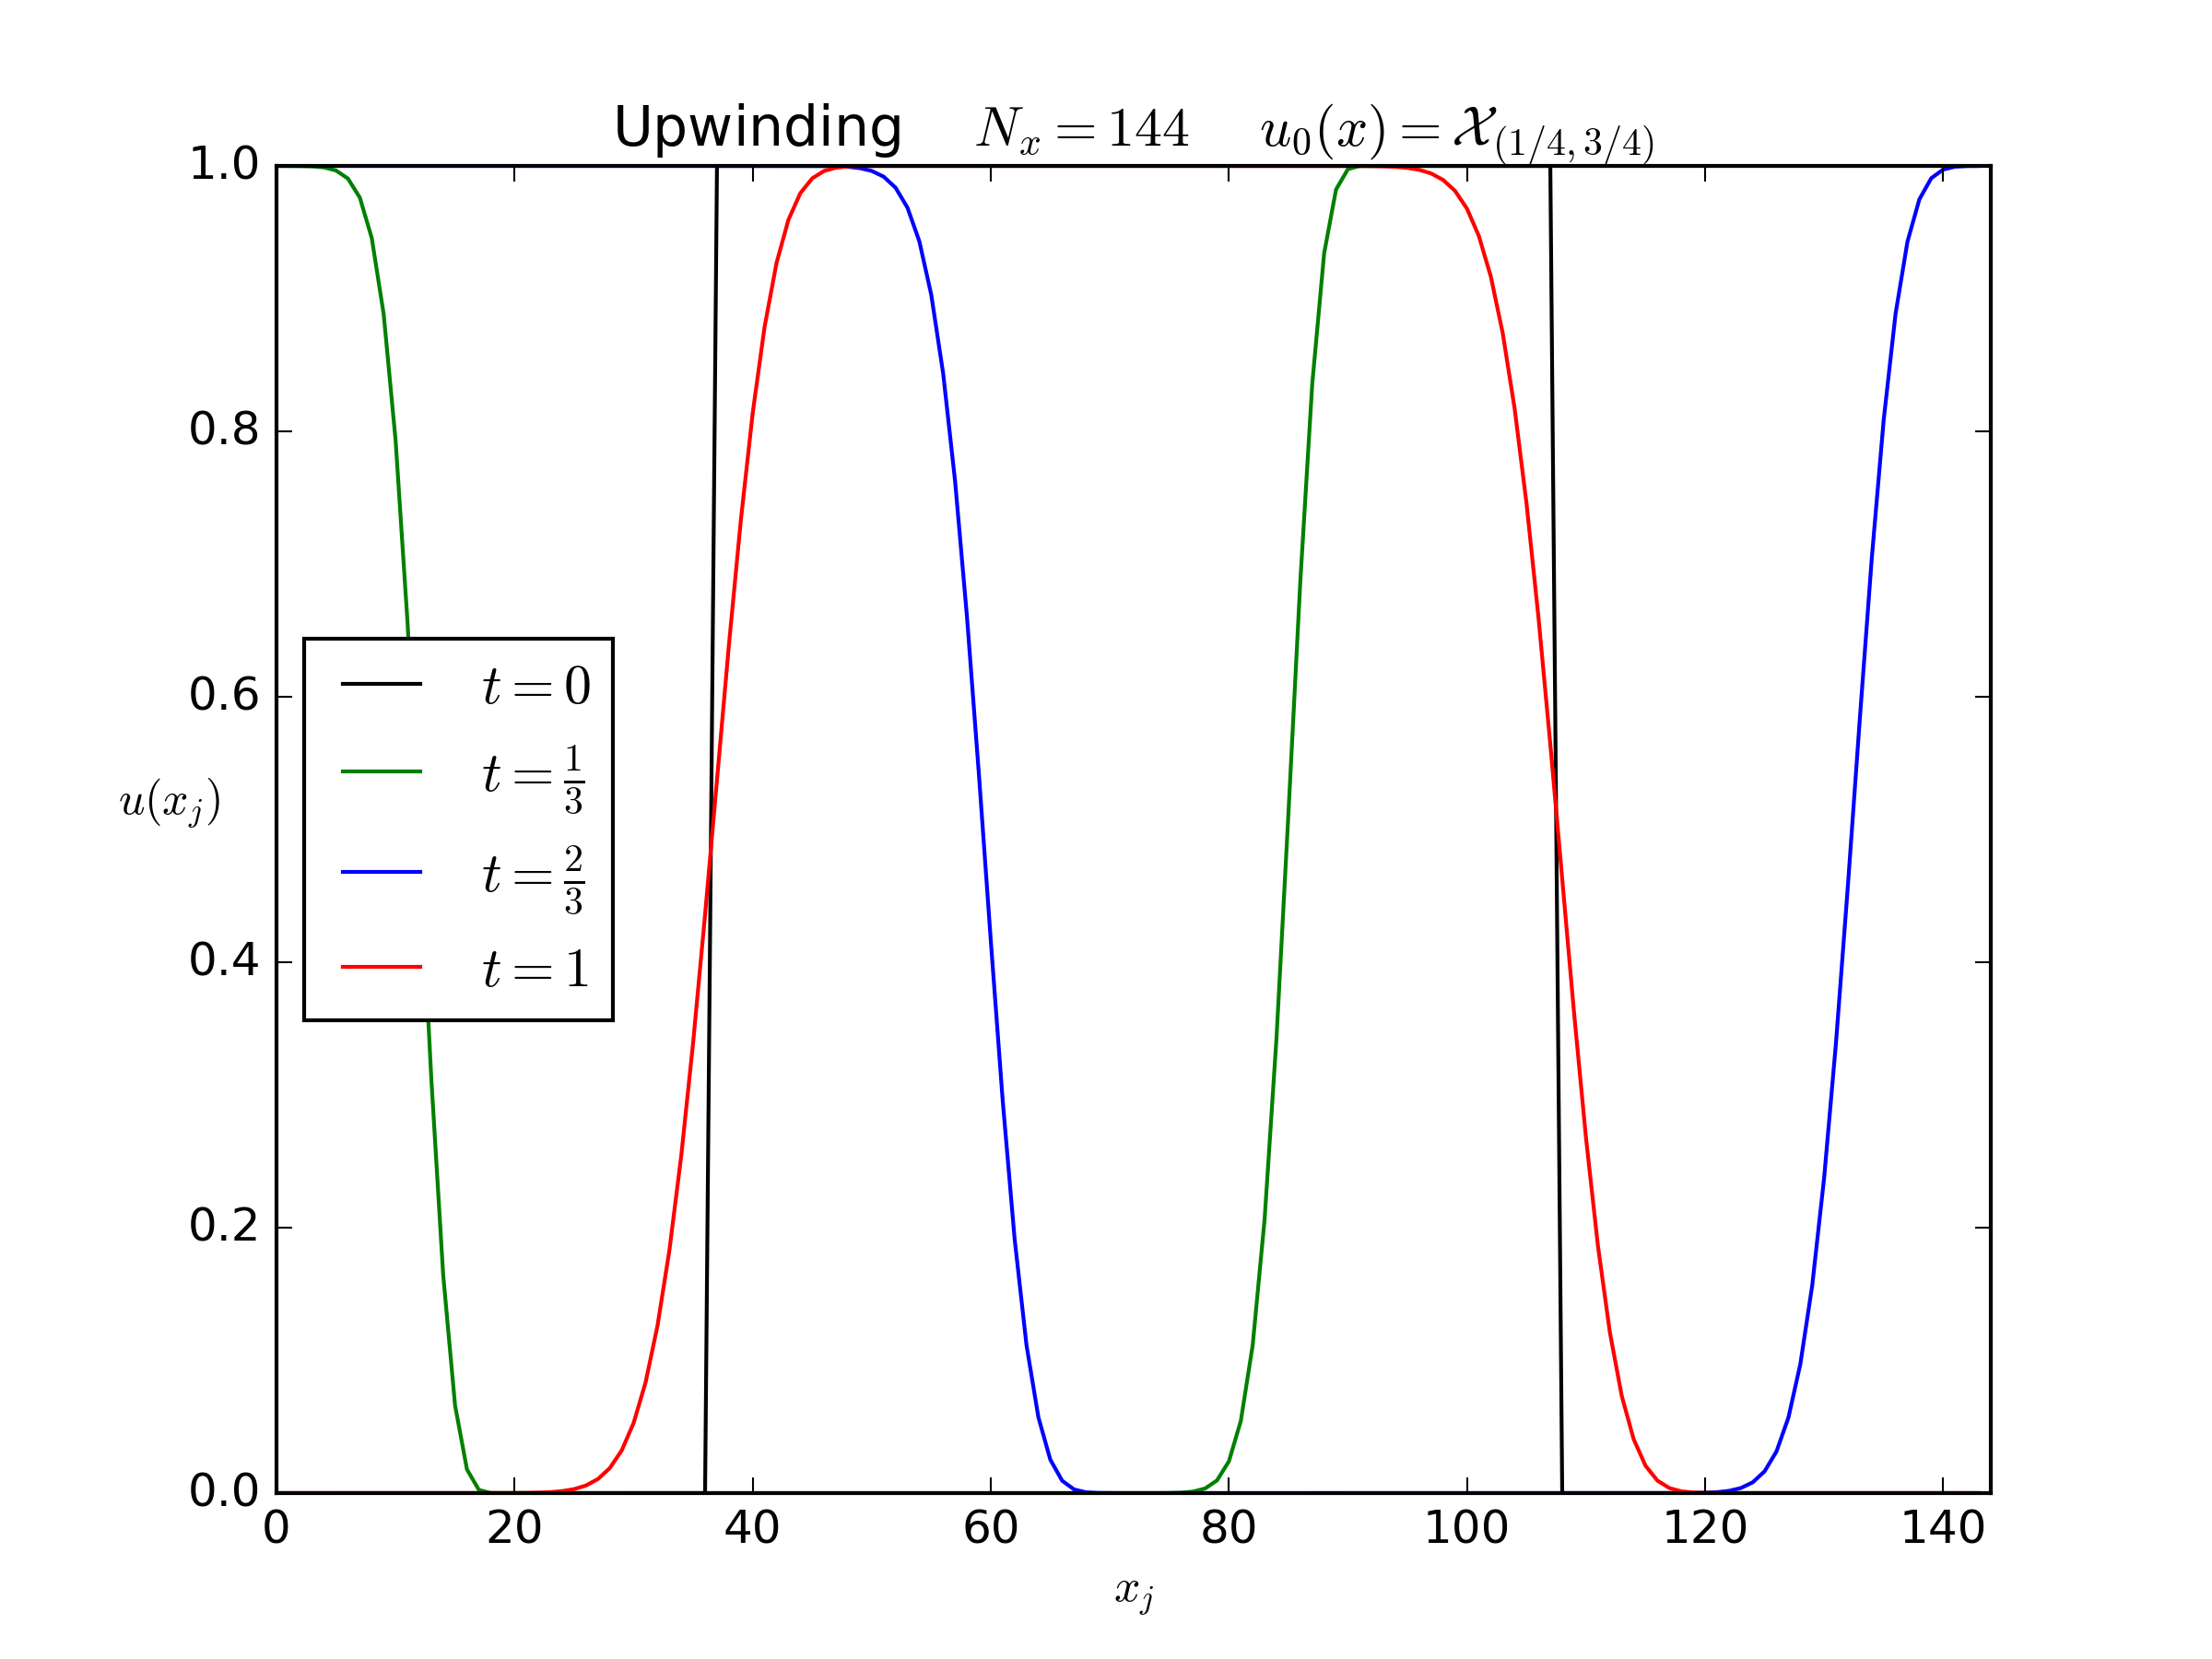
\includegraphics[width=0.45\textwidth]{figures/upwind_discon_snapshots.png}
    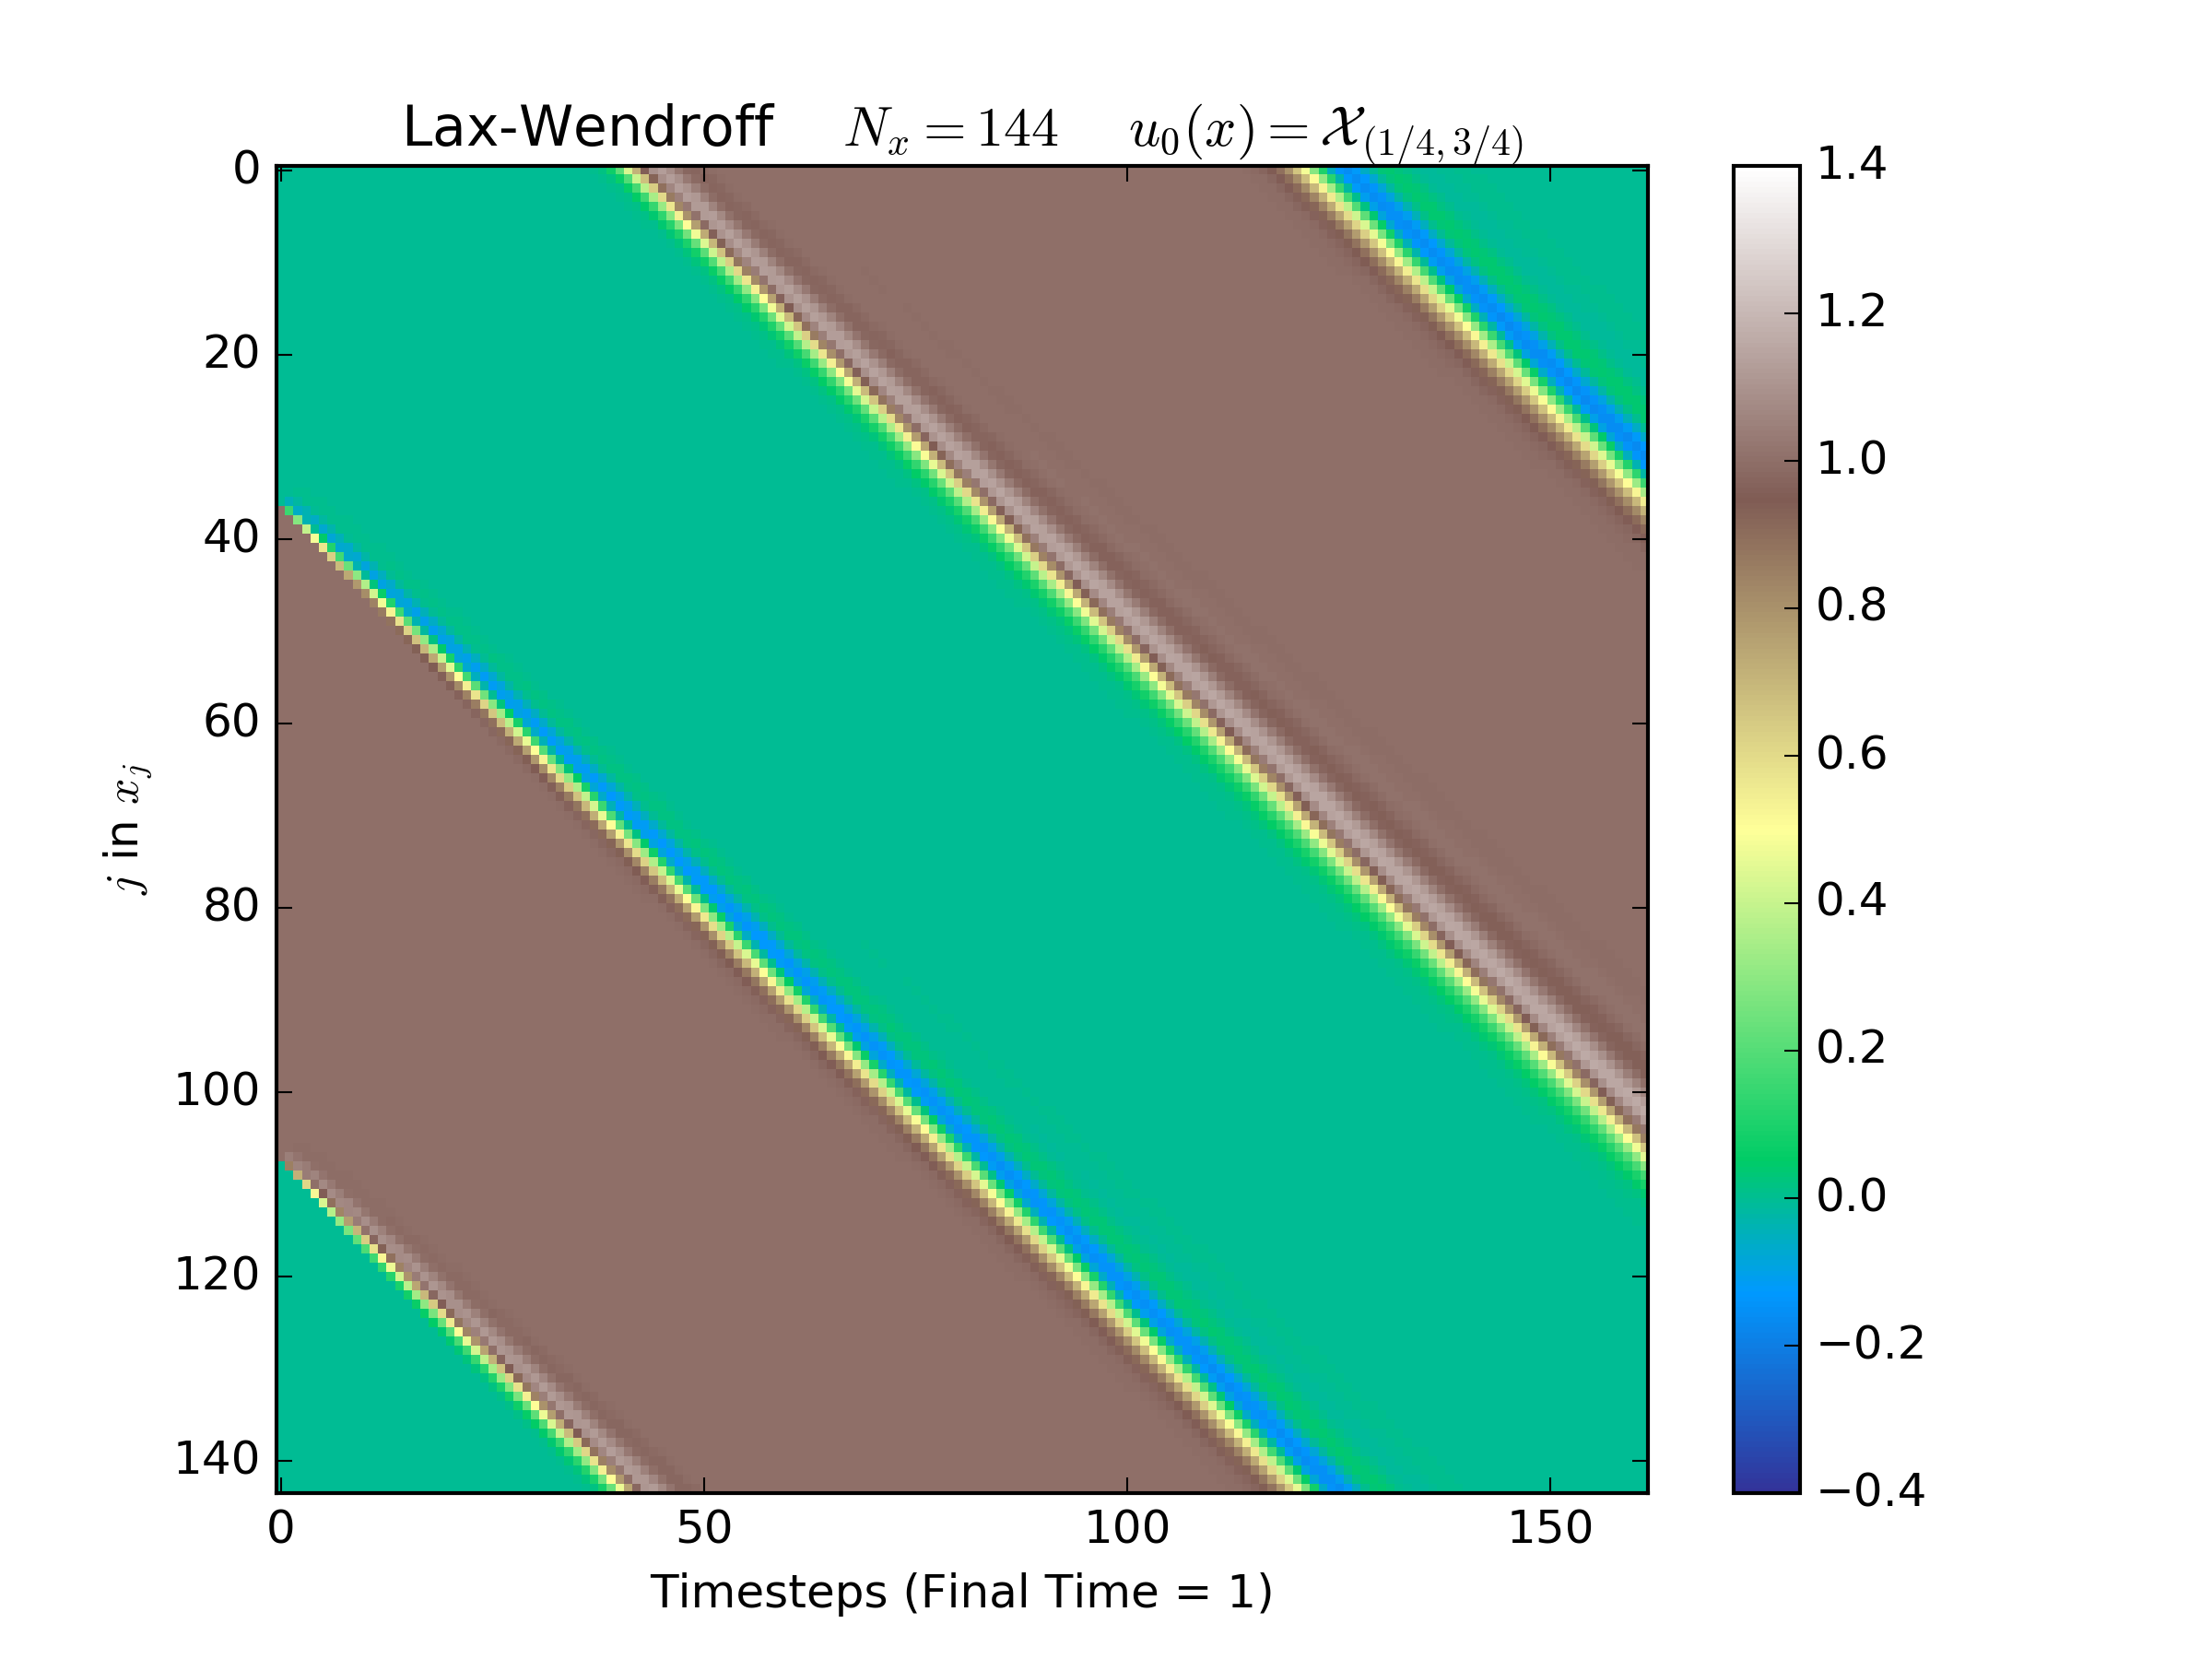
\includegraphics[width=0.45\textwidth]{figures/LW_discon.png}
    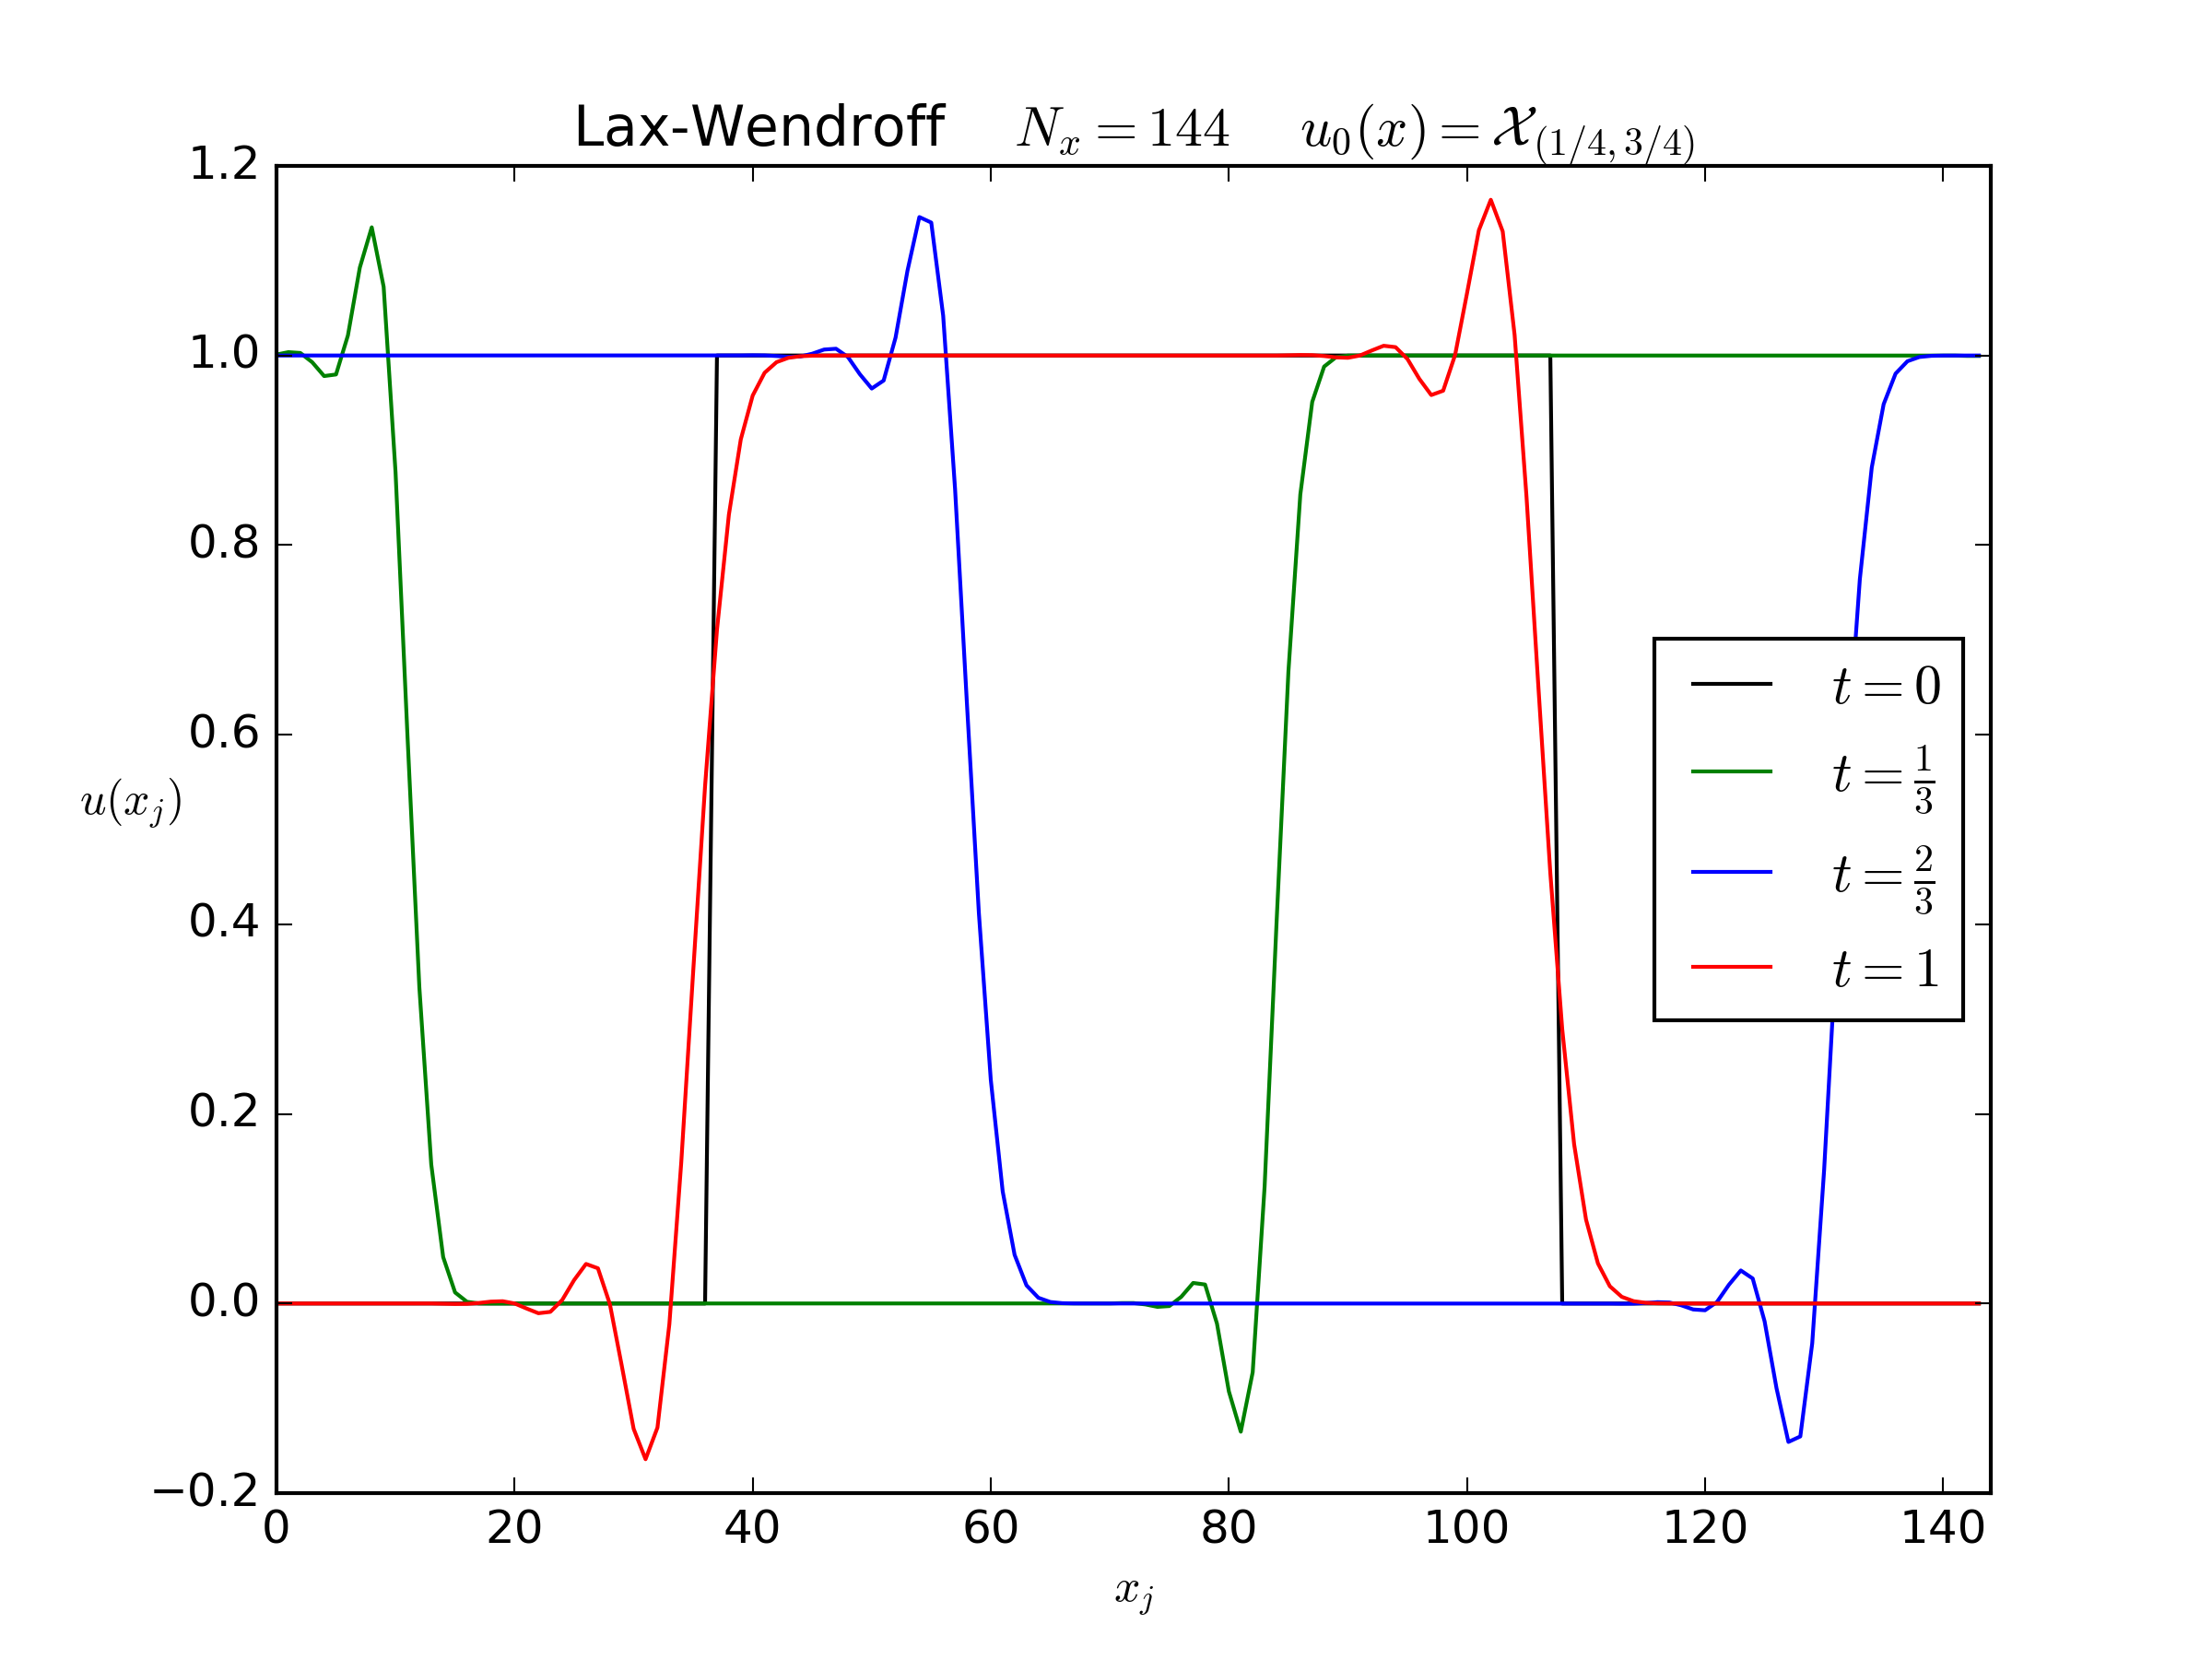
\includegraphics[width=0.45\textwidth]{figures/LW_discon_snapshots.png}
\end{figure}








\FloatBarrier
\pagebreak
\problem{Problem 2}{For solving the heat equation we frequently use Crank-Nicolson, which is trapezoidal rule time integration with a second-order space discretization.  The analogous scheme for the linear advection equation is $$u_j^{n+1} - u_j^n + \frac{\nu}{4}\qty(u_{j+1}^n - u_{j-1}^n) + \frac{\nu}{4}\qty(u_{j+1}^{n+1} - u_{j-1}^{n+1}) = 0,$$ where $\nu = \frac{a\Dt}{\Dx}$.
\begin{enumerate}[\ \ (a)]
    \item Use von Neumann analysis to show that this scheme is unconditionally stable and that $\norm{u^n}_2 = \norm{u^0}_2$.  This scheme is said to be nondissipative - i.e.~there is no amplitude error.  This seems reasonable because this is a property of the PDE.
    \item Solve the advection equation on the periodic domain $[0,1]$ with the initial condition from problem 1b.  Show the solution and comment on your results.
    \item Compute the relative phase as $\frac{\arg(g(\theta))}{-\nu\theta}$, where $g$ is the amplification factor and $\theta = \xi\Dx$, and plot it for $\theta \in [0,\pi]$.  How does the relative phase and lack of amplitude error relate to the numerical solutions you observed in part (b)?
\end{enumerate}}

First note the code used to compute the matrices needed for this scheme:
\lstinputlisting[language=Python, firstline=29, lastline=42]{operators.py}
And here is the method which constructs functions to apply the scheme:
\lstinputlisting[language=Python, firstline=70, lastline=84]{operators.py}
The code for actually solving a problem using this scheme looks similar to the code given in Problem 1, but \verb|step = make_CN_method(Nx,dx,dt,transport_coef)| would replace the line defining \verb|step| through a different scheme.

\begin{enumerate}[\ \ (a)]
    \item
        Let $u_j^n = e^{i\xi x_j}$ and $u_j^{n+1} = g(\xi)u_j^n$.  Then
        \begin{align*}
            g(\xi)e^{i\xi x_j} - e^{i\xi x_j} + \frac{\nu}{4}\qty(e^{i\xi x_j}e^{i\xi\Dx} - e^{i\xi x_j}e^{-i\xi\Dx}) + \frac{\nu}{4}\qty(g(\xi)e^{i\xi x_j}e^{i\xi\Dx} - g(\xi)e^{i\xi x_j}e^{-i\xi\Dx}) &= 0 \\
            g(\xi) - 1 + \frac{\nu}{4}\qty(e^{i\xi\Dx} - e^{-i\xi\Dx}) + g(\xi)\frac{\nu}{4}\qty(e^{i\xi\Dx} - e^{-i\xi\Dx}) &= 0 \\
            g(\xi) = \frac{1 - \dfrac{\nu}{2}\cdot\dfrac{e^{i\xi\Dx} - e^{-i\xi\Dx}}{2}}{1 + \dfrac{\nu}{2}\cdot\dfrac{e^{i\xi\Dx} - e^{-i\xi\Dx}}{2}}&
        \end{align*}
        Since $i\sin(\theta) = \frac{1}{2}\qty(e^{i\theta} - e^{-i\theta})$, then, with $\theta \coloneqq \xi\Dx$,
        \begin{align*}
            g(\theta) = \frac{1 - i\frac{\nu}{2}\sin(\theta)}{1 + i\frac{\nu}{2}\sin(\theta)} = \frac{\qty(1 - i\frac{\nu}{2}\sin(\theta))^2}{1 + \frac{\nu^2}{4}\sin^2(\theta)} = \frac{1 - \frac{\nu^2}{4}\sin^2(\theta)}{1 + \frac{\nu^2}{4}\sin^2(\theta)} - i\frac{\nu\sin(\theta)}{1 + \frac{\nu^2}{4}\sin^2(\theta)}
        \end{align*}
        For ease, let $A = 1 - \frac{\nu^2}{4}\sin^2(\theta)$, $B = \nu\sin(\theta)$, and $C = 1 + \frac{\nu^2}{4}\sin^2(\theta)$.  Then
        \begin{align*}
            g(\theta) = \frac{A}{C} - i\frac{B}{C}
        \end{align*}
        So,
        \begin{align*}
            \abs{g(\theta)}^2 = \frac{A^2 + B^2}{C^2}
        \end{align*}
        But since
        \begin{align*}
            A^2 + B^2 = 1 - \frac{\nu^2}{2}\sin^2(\theta) + \frac{\nu^4}{16}\sin^4(\theta) + \nu^2\sin^2(\theta) = 1 + \frac{\nu^2}{2}\sin^2(\theta) + \frac{\nu^4}{16}\sin^4(\theta) = C^2
        \end{align*}
        Which proves $\abs{g}^2 = 1$, showing the scheme is unconditionally stable.  This means we can show
        \begin{align*}
            \norm{u^n}_2 = \norm{g(\xi)^nu^0}_2 = \abs{g(\xi)}^n\norm{u^0}_2 = 1\cdot\norm{u^0}_2 = \norm{u^0}_2,
        \end{align*}
        which implies the scheme is non-dissipative.
    \item
        Below is an image of the solution of the advection equation on the periodic domain using the ``Crank Nicolson for Advection'' scheme.
        \begin{figure}[ht!]
            \centering
            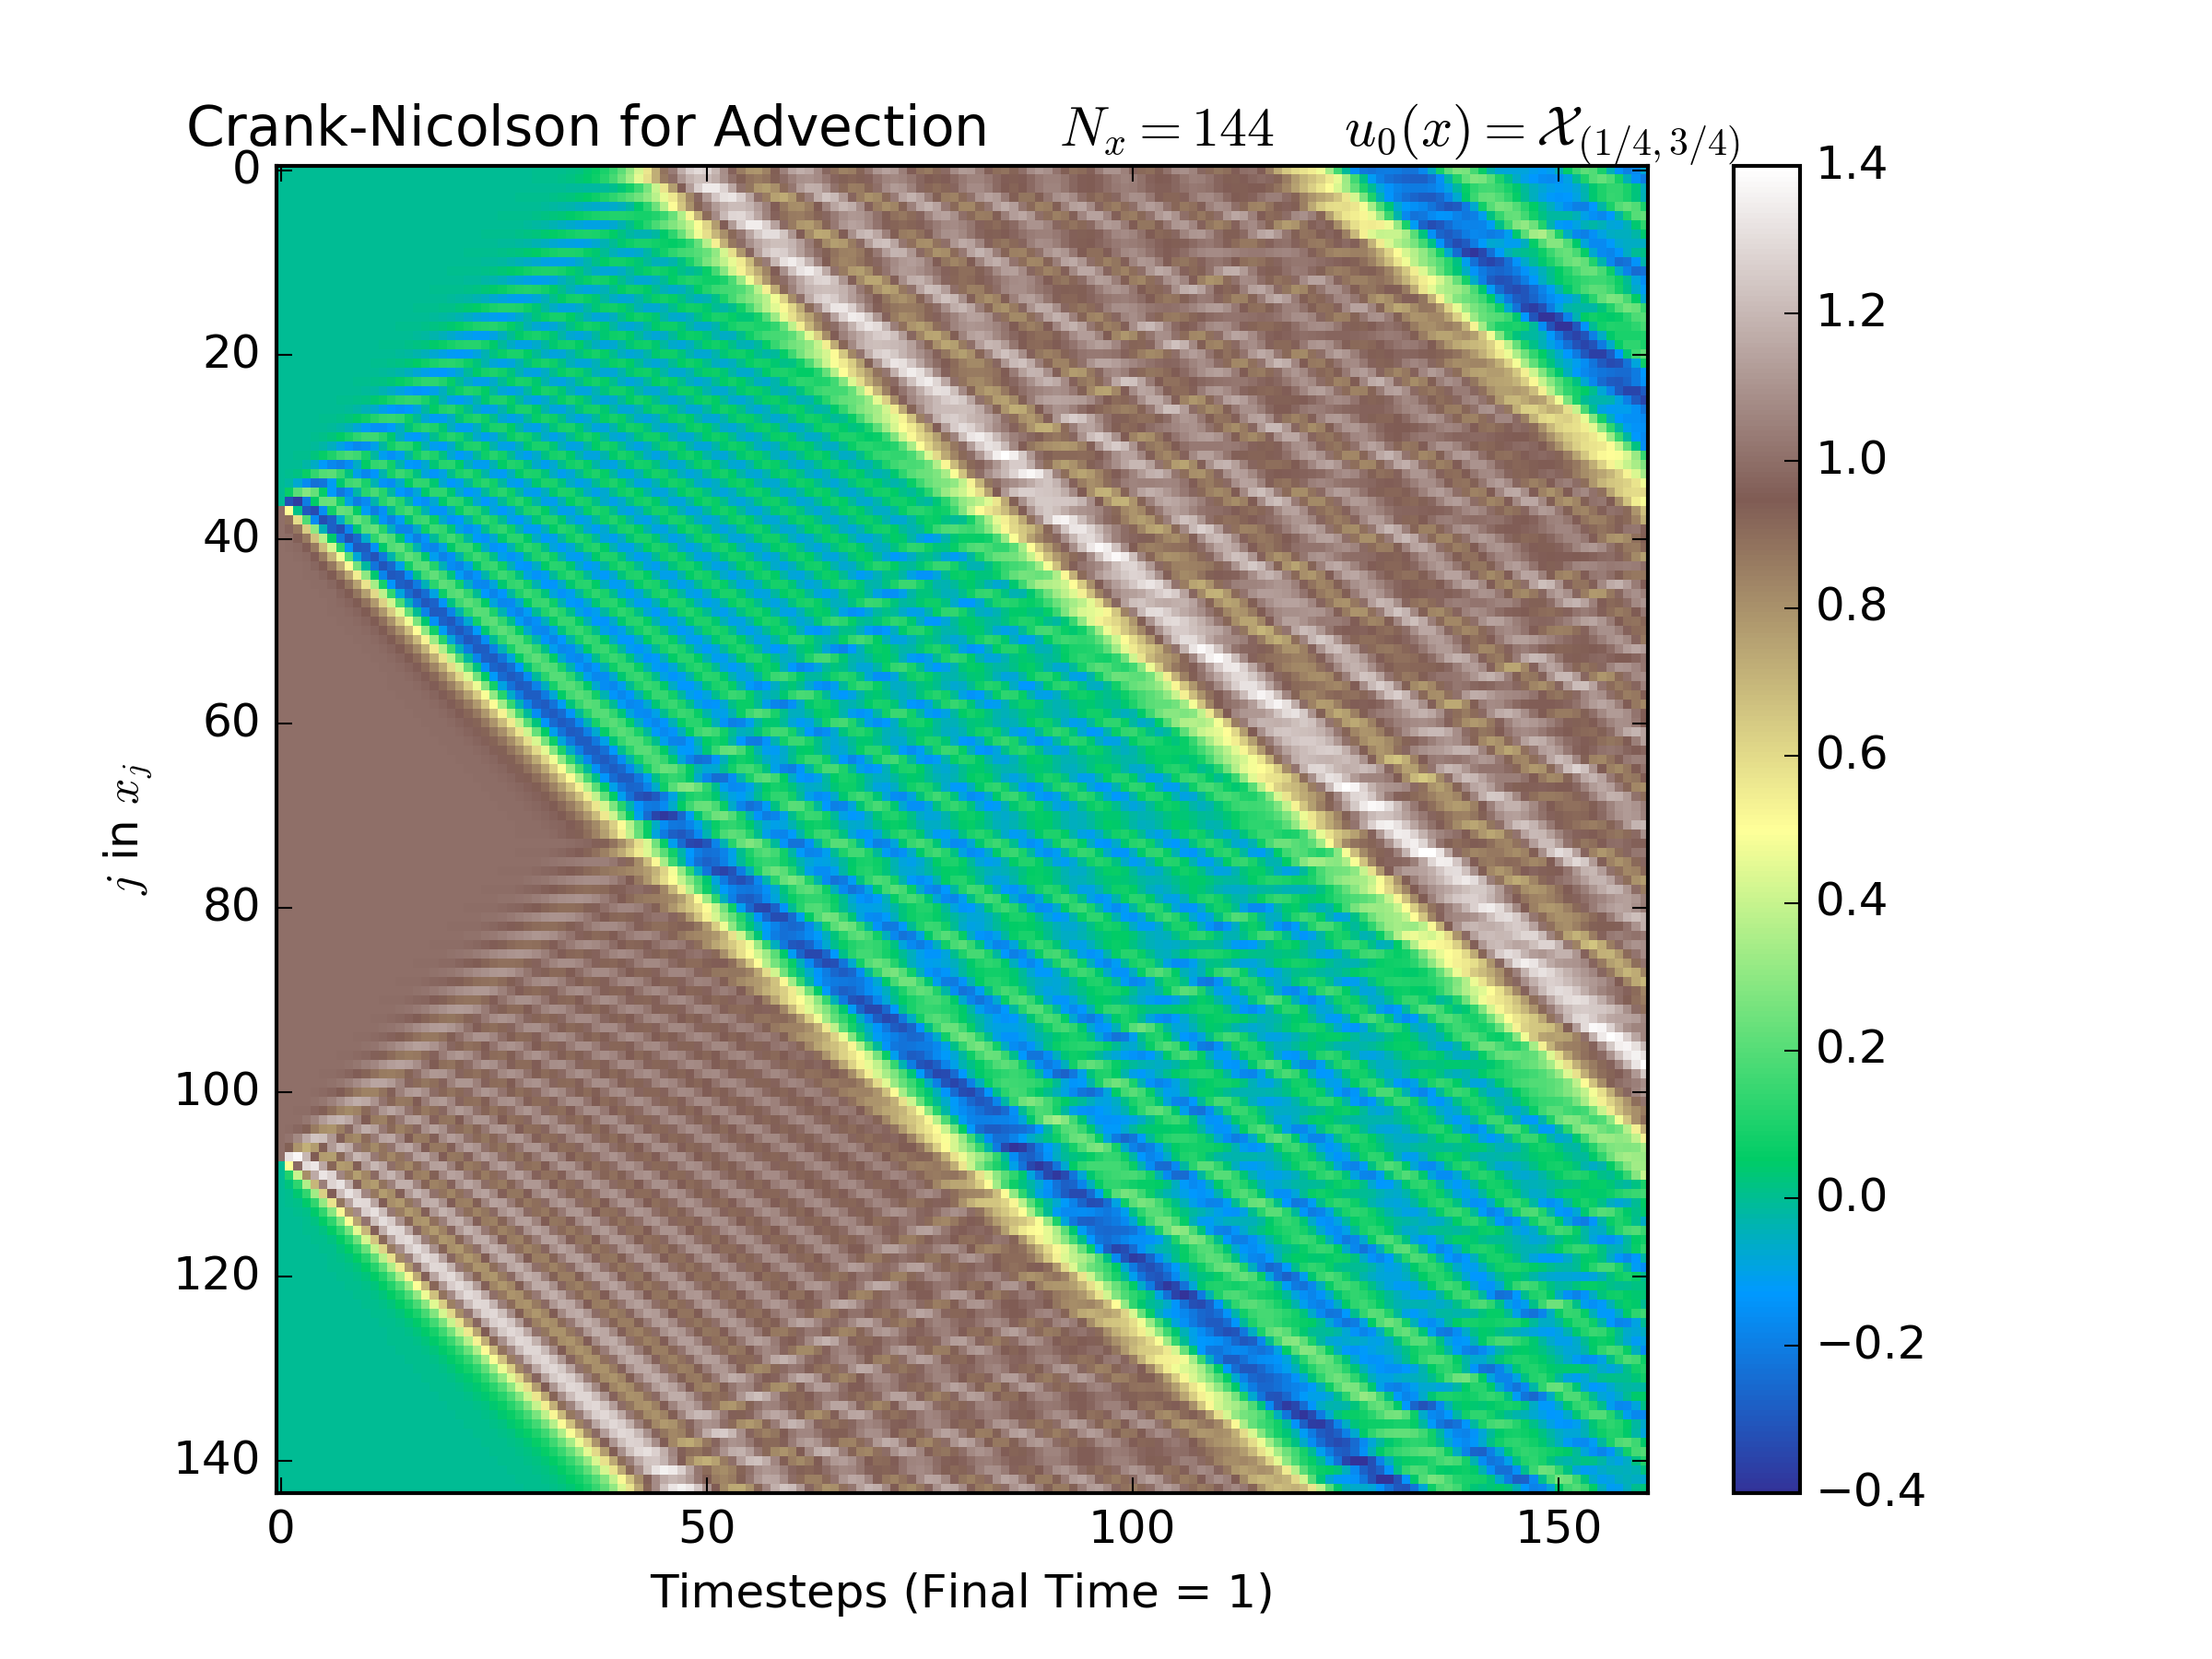
\includegraphics[width=0.45\textwidth]{figures/CN_discon.png}
            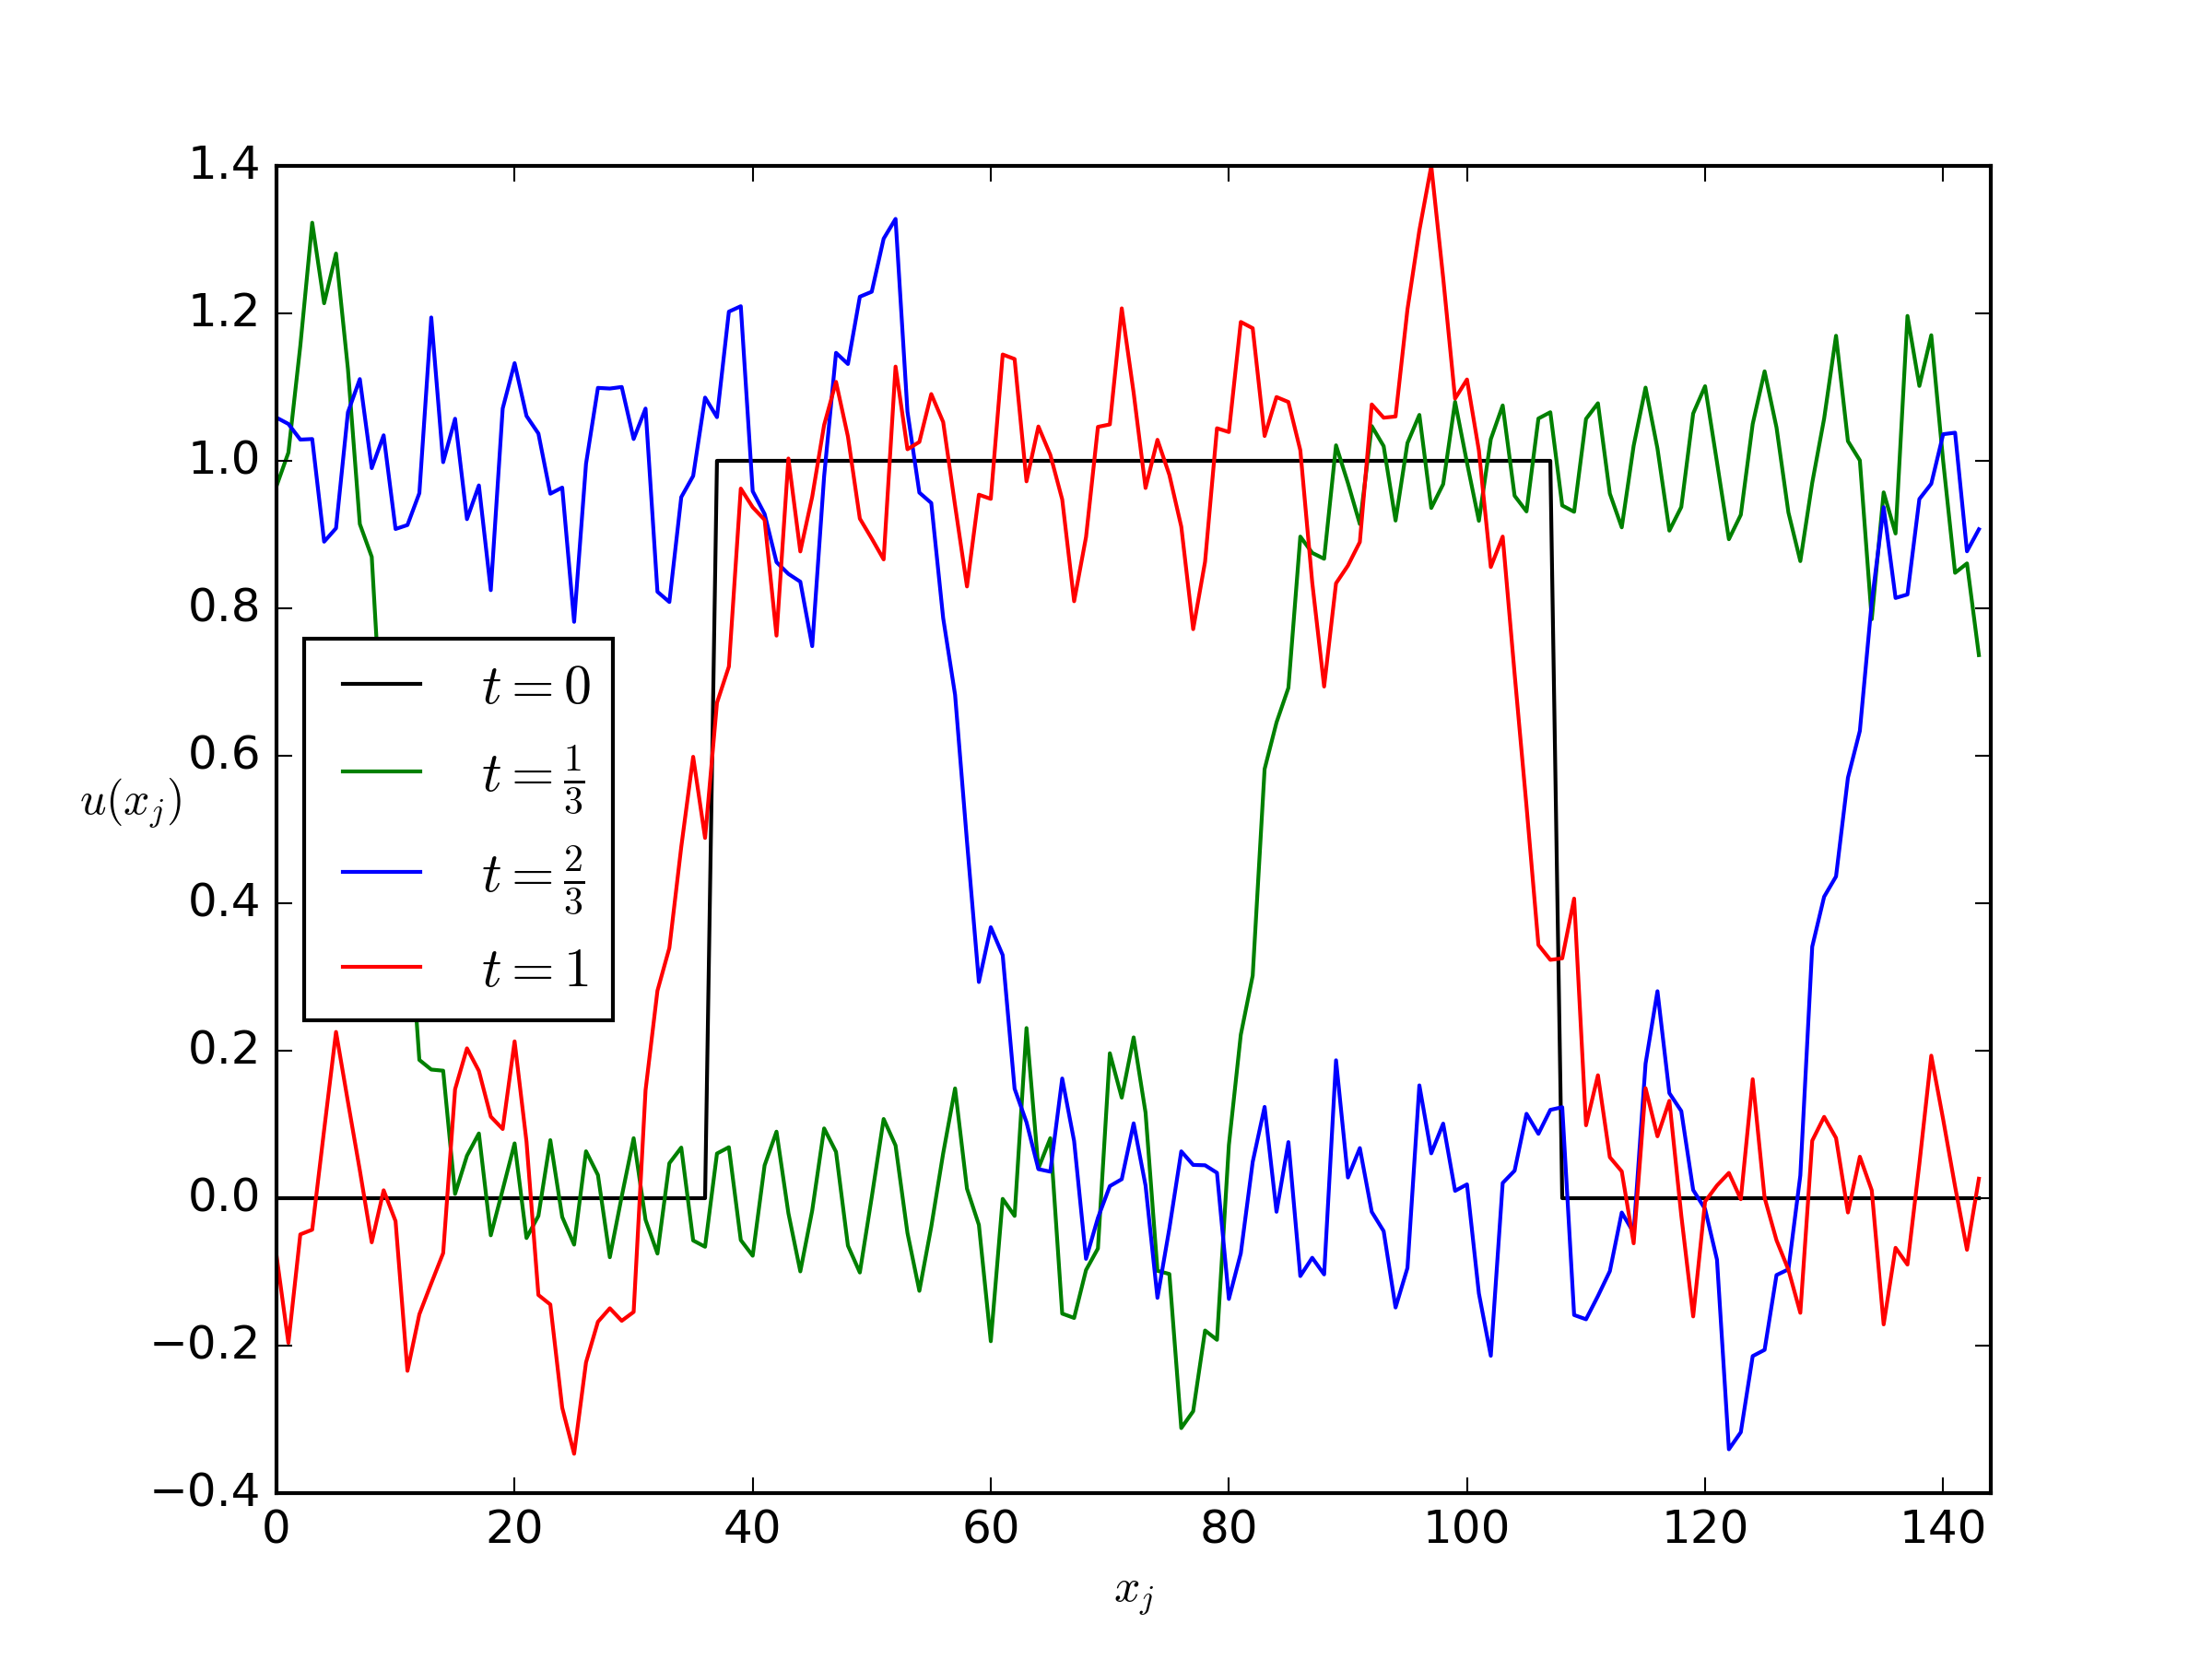
\includegraphics[width=0.45\textwidth]{figures/CN_snapshots.png}
        \end{figure}
        \FloatBarrier
    \item
        We can explicitly write $\arg(g(\theta))$ as $$\arg(g(\theta)) = \arg(\frac{A}{C} - i\frac{B}{C}) = \tan^{-1}\qty(-\frac{B}{A}) = \tan^{-1}\qty(\frac{-\nu\sin(\theta)}{1 - \frac{\nu^2}{4}\sin^2(\theta)}).$$ Thus the relative phase $\frac{\arg(g(\theta))}{-\nu\theta}$ is
        \begin{align*}
            \frac{\arg(g(\theta))}{-\nu\theta} &= -\frac{1}{\nu\theta}\arctan\qty(\frac{-\nu\sin(\theta)}{1 - \frac{\nu^2}{4}\sin^2(\theta)})
        \end{align*}
        which for $\nu = 0.9$, is
        \begin{align*}
            \frac{\arg(g(\theta))}{-0.9\theta} &= -\frac{1}{0.9\theta}\arctan\qty(\frac{-0.9\sin(\theta)}{1 - \frac{0.9^2}{4}\sin^2(\theta)})
        \end{align*}
        which looks like
        \begin{figure}[ht!]
            \centering
            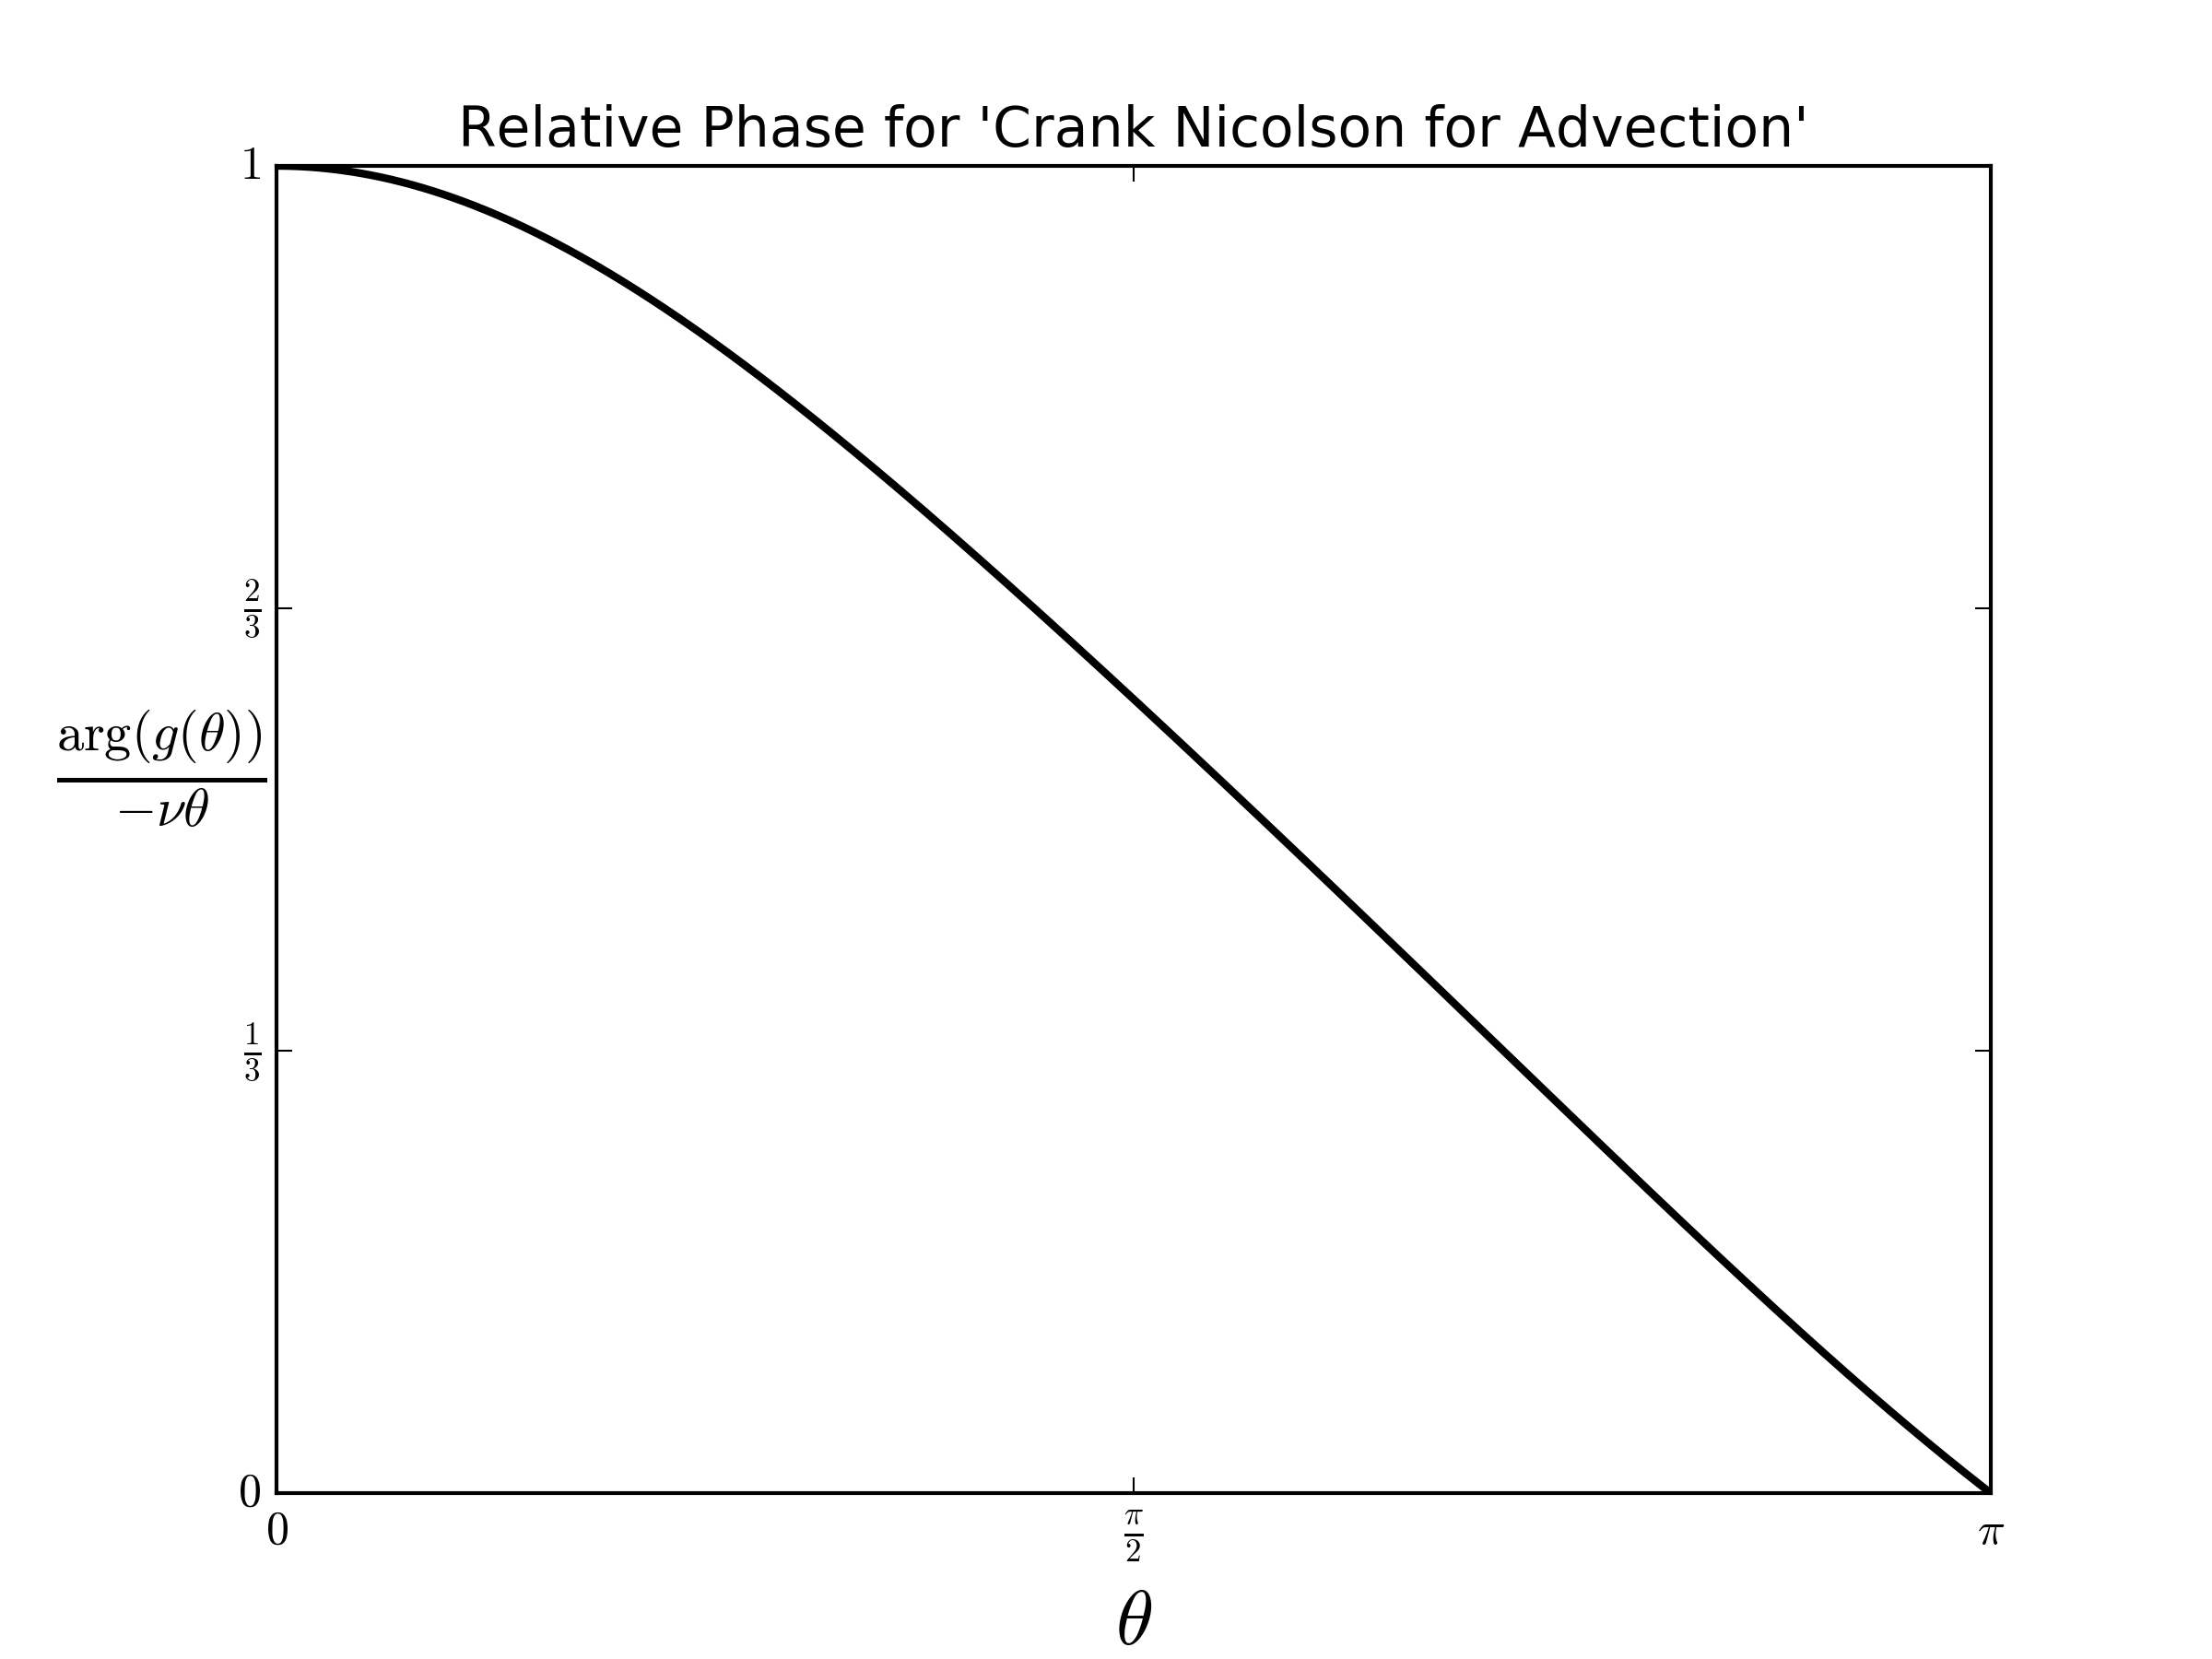
\includegraphics[width=\textwidth]{figures/relative_phase.png}
        \end{figure}
        \FloatBarrier
        This means the highest frequencies move much slower than the lowest frequencies.  Since the step function is the superposition of many different frequencies, we see what seems to produce backward movement near the discontinuities, but in reality it is slow, forward-moving frequencies.  The above graph shows the scheme is highly dispersive since there are big differences between relative phases for different fequencies.

\end{enumerate}








\end{document}









